\documentclass[12pt]{article}
\usepackage{graphicx}
\usepackage{amsmath}
\usepackage{amssymb}
\usepackage{color}
\usepackage{braket}
\usepackage[margin=1in]{geometry}
\usepackage{mathtools}
\usepackage{tikz}

\allowdisplaybreaks
\numberwithin{equation}{section}

\interfootnotelinepenalty=10000

\usepackage{calligra}
\usepackage{hyperref}
\hypersetup{colorlinks=true, linkcolor=blue}

\DeclareMathAlphabet{\mathcalligra}{T1}{calligra}{m}{n}
\DeclareFontShape{T1}{calligra}{m}{n}{<->s*[2.2]callig15}{}
\newcommand{\scriptr}{\mathcalligra{r}\,}
\newcommand{\boldscriptr}{\pmb{\mathcalligra{r}}\,}

\newcommand{\Lagr}{\mathcal{L}}
\newcommand{\Hami}{\mathcal{H}}
\newcommand{\reals}{\rm I\!R}
\newcommand{\order}{\mathcal{O}}
\newcommand{\bx}{\mathbf{x}}
\newcommand{\bp}{\mathbf{p}}
\newcommand{\bq}{\mathbf{q}}
\newcommand{\redtext}[1]{\textcolor{red}{#1}}
\newcommand{\pvec}[1]{\vec{#1}\mkern2mu\vphantom{#1}}

\setcounter{section}{-1}


\begin{document}
	\title{Numerical Relativity Project \#2}
	\author{Alex Pandya}
	\date{June 20th, 2018}
	\maketitle

\section{Background}
In this project we aim to solve the equations of motion for a self-gravitating scalar field in spherical symmetry.  The key difference between this project and the previous one is that we now care about how the scalar field modifies the spacetime it occupies, whereas in the previous project we used a static Schwarzschild spacetime.

The spherically symmetric line element in isotropic (conformally flat) form is given by
\begin{equation} \label{eq:line_element}
ds^2 = -(\alpha^2 - \psi^4 \beta^2) dt^2 + 2 \psi^4 \beta dr dt + \psi^4 [dr^2 + r^2 (d\theta^2 + \sin^2 \theta d\phi^2)],
\end{equation}
where $\alpha(r, t)$ is called the \textit{lapse function}, $\beta(r, t)$ is the \textit{shift} (which is the radial component of the \textit{shift vector}; the other components are zero), and $\psi(r, t)$ is the \textit{conformal factor}.

In this formalism, the Klein-Gordon equation for the scalar field $\Phi(r, t)$ may be written in terms of auxiliary variables $\xi$ and $\Pi$, defined to be:
\begin{align}
\xi(r, t) &= \Phi' \label{eq:xi_defn} \\
\Pi(r, t) &= \frac{\psi^2}{\alpha}(\dot{\Phi} - \beta \xi), \label{eq:Pi_defn} 
\end{align}
where throughout this document a dot $(\dot{~})$ denotes a partial derivative with respect to $t$, and a prime $(')$ denotes a partial derivative with respect to $r$.  Using these auxiliary variables, we can derive a closed system of equations for the quantities of interest ($\xi, \Pi, \psi, \alpha, \beta$).

The first equation of this system is the hyperbolic Klein-Gordon equation\footnote{Note that this equation differs from that in the sample code.  The sample code has an additional factor of $1/2$ in the $3r\psi'/\psi$ term, which I believe to be in error.}
\begin{equation} \label{eq:hyperbolic_KGE}
\dot{\Pi} - \frac{1}{r^2 \psi^4} \Big[ r^2 \psi^4 \Big( \beta \Pi + \frac{\alpha \xi}{\psi^2} \Big)\Big]' + \frac{2}{3} \Pi \Big[ \beta' + \frac{2 \beta}{r} \Big(1 + \frac{3 r \psi'}{\psi} \Big) \Big] = 0,
\end{equation}
followed by the hyperbolic evolution equation for $\xi$:
\begin{equation} \label{eq:xi_evol}
\dot{\xi} - \Big( \frac{\alpha \Pi}{\psi^2} + \beta \xi \Big)' = 0,
\end{equation}
the Hamiltonian constraint equation, which we will use as an elliptic constraint for $\psi$
\begin{equation} \label{eq:psi_evol}
\psi'' + \psi' \frac{2}{r} + \frac{\psi^5}{12} \Big[ \frac{1}{\alpha} \Big( \beta' - \frac{\beta}{r} \Big)^2 \Big] + \pi \psi [\xi^2 + \Pi^2] = 0,
\end{equation}
the momentum constraint equation, an elliptic equation for $\beta$
\begin{equation} \label{eq:beta_evol}
\beta'' + \Big( \beta' - \frac{\beta}{r} \Big) \Big[ \frac{2}{r} + \frac{6 \psi'}{\psi} - \frac{\alpha'}{\alpha} \Big] + \frac{12 \pi \alpha \xi \Pi}{\psi^2} = 0,
\end{equation}
and the maximal slicing condition yields an elliptic equation for $\alpha$:
\begin{equation} \label{eq:alpha_evol}
\alpha'' + \alpha' \Big[ \frac{2}{r} + \frac{2 \psi'}{\psi} \Big] - \alpha^{-1} \Big[ \frac{2 \psi^4}{3} \Big( \beta' - \frac{\beta}{r} \Big)^2 \Big] - 8 \pi \alpha \Pi^2 = 0.
\end{equation}

Setting the trace of the extrinsic curvature equal to zero (the maximal slicing condition itself) yields a hyperbolic equation for the conformal factor:
\begin{equation} \label{eq:psi_hyperbolic_eqn}
\dot{\psi} - \beta \Big( \frac{\psi}{3 r} + \psi' \Big) - \frac{\psi \beta'}{6} = 0,
\end{equation}
which may be used to evolve $\psi$, but only after the initial timestep is solved for using the $\psi$ elliptic equation in order to ensure that the initial conditions are consistent.

All of the above equations are derived from the ADM equations in the appendix.

\section{Problem 1}
This problem asks us to verify the boundary conditions on the quantities of interest ($\xi, \Pi, \psi, \alpha, \beta$) at $r = 0$, to ensure that they are regular and finite there.

Expanding out equation \ref{eq:hyperbolic_KGE}, we get:
\begin{equation}
\begin{aligned}
0 &= \dot{\Pi} - \Big[ \frac{2 \beta \Pi}{r} + \frac{4 \psi' \beta \Pi}{\psi} + \beta' \Pi + \beta \Pi' + \frac{2 \alpha \xi}{r \psi^2} + \frac{2 \psi' \alpha \xi}{\psi^3} + \frac{\alpha' \xi}{\psi^2} + \frac{\alpha \xi'}{\psi^2} \Big] \\
&+ \frac{2}{3} \Pi \Big[ \beta' + \frac{2 \beta}{r} \Big(1 + \frac{3 r \psi'}{\psi} \Big) \Big]; \\
\end{aligned}
\end{equation}
inspection of this equation implies that in order for it to be regular and finite at $r = 0$, we must require $\beta \Pi \to 0$ and $\alpha \xi \to 0$ as $r \to 0$.  We need more equations to constrain the behavior further.

Expanding out equation \ref{eq:xi_evol} doesn't help us, so we can determine most of the other conditions simply by inspection of equations \ref{eq:psi_evol} - \ref{eq:alpha_evol}.  The second term in equation \ref{eq:psi_evol} implies that $\psi' \to 0$ as $r \to 0$, and the term inside both brackets and parentheses implies $\beta \to 0$ as $r \to 0$.  Equation \ref{eq:alpha_evol}'s second term implies $\alpha' \to 0$ as $r \to 0$.  Now that we know these things, the constraint on $\alpha'$ implies that $\alpha$ will not be constrained, so from the paragraph above we know that $\xi \to 0$.  

So far, we have:
\begin{equation*}
\begin{aligned}
\beta  (r=0, t) &= 0 \\
\xi    (r=0, t) &= 0 \\
\psi'  (r=0, t) &= 0 \\
\alpha'(r=0, t) &= 0,
\end{aligned}
\end{equation*}
but we still need an equation for $\Pi$ or $\Pi'$ to fully constrain the system.  Looking at the definition of $\Pi$ in equation \ref{eq:Pi_defn}, we can see that as $r \to 0$ the second term drops out, but we don't know anything about the first term.  Let's try taking a derivative with respect to $r$, and see what falls out:
\begin{equation*}
\begin{aligned}
\Pi' &= \Big[ \psi^2 \alpha^{-1} \dot{\phi} - \psi^2 \alpha^{-1} \beta \xi \Big]' \\
&= 2 \psi \psi' \alpha^{-1} \dot{\phi} - \psi^2 \alpha^{-2} \alpha' \dot{\phi} + \psi^2 \alpha^{-1} \dot{\phi}' \\
&- 2 \psi \psi' \alpha^{-1} \beta \xi + \psi^2 \alpha^{-2} \alpha' \beta \xi - \psi^2 \alpha^{-1} \beta' \xi - \psi^2 \alpha^{-1} \beta \xi';
\end{aligned}
\end{equation*}
applying the constraints we already know for when $r \to 0$, we find:
\begin{equation*}
\begin{aligned}
\Pi'(r=0, t) &= \psi^2 \alpha^{-1} \dot{\phi}' \\
&= \psi^2 \alpha^{-1} \partial_r (\partial_t \phi) \\
&= \psi^2 \alpha^{-1} \partial_t (\partial_r \phi) \\
&= \psi^2 \alpha^{-1} \partial_t (\xi) \\
&= \psi^2 \alpha^{-1} \partial_t (0) \\
&= 0,
\end{aligned}
\end{equation*}
so in summary, at $r = 0$, we have the full set of conditions
\begin{equation}
\begin{aligned}
\beta  (r=0, t) &= 0 \\
\xi    (r=0, t) &= 0 \\
\psi'  (r=0, t) &= 0 \\
\alpha'(r=0, t) &= 0 \\
\Pi'   (r=0, t) &= 0,
\end{aligned}
\end{equation}
as we were asked to show.

\section{Problem 2}
In this problem we are asked to derive boundary conditions to be applied at the outer boundary ($r = R$) which do not couple matter variables ($\Pi, \xi$) or space variables ($\alpha, \beta, \psi$) amongst themselves or to each other.  We are told to define the space variable boundary conditions such that they are consistent to $O(1/r^2)$ with asymptotic flatness (which we should expect for large $R$), which means we should have conditions with solutions of the form
\begin{equation} \label{eq:space_var_outer_behavior}
\begin{aligned}
\psi   &= 1 + \frac{a_0(t)}{r} + O(1/r^2) \\
\alpha &= 1 + \frac{b_0(t)}{r} + O(1/r^2) \\
\beta  &= 0 + \frac{c_0(t)}{r} + O(1/r^2),
\end{aligned}
\end{equation}
where the leading order behavior is determined by the asymptotic behavior of the space variable (e.g. by comparing the metric \ref{eq:line_element} to the Minkowski metric).

We have to enforce the above behavior on our variables somehow and write constraint equations.  Taking a derivative with respect to $r$ of the above equations, we find:
\begin{align}
\psi' + \frac{\psi - 1}{r}     &= 0 \\
\alpha' + \frac{\alpha - 1}{r} &= 0 \\
\beta' + \frac{\beta}{r}       &= 0,
\end{align} 
which we will enforce as our outer boundary condition on these variables\footnote{I don't like the description for this problem very much.  I think it's important to state that for these boundary conditions we're trying to write down constraint equations which force $\{\psi, \alpha, \beta\}$ to obey equation \ref{eq:space_var_outer_behavior}.}.

Now we need boundary conditions for the matter variables $\xi$ and $\Pi$.  We are asked to force these variables to be consistent with the outgoing radiation condition to $O(1/r^2)$.  Applying the outgoing radiation condition to the matter variables, we have:
\begin{equation}
\begin{aligned}
0 &= \partial_t (r \xi) + \partial_r (r \xi) \\
&= r \partial_t \xi + r \partial_r \xi + \xi \\
&= r \dot{\xi} + r \xi' + \xi \\
&= \dot{\xi} + \xi' + \frac{\xi}{r}.
\end{aligned}
\end{equation}
following the exact same procedure for $\Pi$, we find
\begin{equation}
0 = \dot{\Pi} + \Pi' + \frac{\Pi}{r}.
\end{equation}
Since we directly used the outgoing radiation condition to derive these equations, they are guaranteed to be consistent with the outgoing radiation condition to any order in $1/r$.

These boundary conditions have been verified by comparison with those coded up in the sample code for this project\footnote{Sample code which solves problems 1-5: \url{http://physics.princeton.edu/~fpretori/group_resources/PiTP_2009/emkg_5.tar.gz}} and by taking the spherical-symmetry special case of the boundary conditions\footnote{The outer boundary conditions can be found in equation 9 of \url{https://arxiv.org/pdf/gr-qc/0508110.pdf}.  These equations may be converted to spherical coordinates by noting that $r = \sqrt{\rho^2 + z^2}$, and converting the $\rho$ and $z$ derivatives to be $r$ derivatives.} in a paper describing an axisymmetric self-gravitating scalar field code \cite{Pretorius06}, though in the latter they use Dirichlet boundary conditions for $\alpha, \beta$ rather than the Robin conditions we use here.

\section{Problem 3}
In this problem we are asked to write code to solve the Klein-Gordon equation in the form of equations \ref{eq:hyperbolic_KGE} - \ref{eq:xi_evol} to integrate $\Pi$ and $\xi$ for a flat space background.  We are also asked to use equation \ref{eq:Pi_defn} to integrate the scalar field $\Phi$.  The problem statement tells us to use a second-order Crank-Nicolson scheme, and to implement Kreiss-Oliger (KO) dissipation near the origin.

To begin, we must note that the flat space background part of the problem statement implies that we can take the zeroth order behavior of equation \ref{eq:space_var_outer_behavior} to set the values of the space variables, namely: $\psi = \alpha = 1$ and $\beta = 0$.  We initialize the matter variables with $\Phi$ a Gaussian, $\xi = \Phi'$.  To set $\Pi$, we use the ``as in-going as possible" condition on the matter, namely $\dot{\Phi} = \Phi'$.  In flat space our matter variables become
\begin{equation*}
\begin{aligned}
\xi_{\mathrm{flat~space}} &= \Phi' \\
\Pi_{\mathrm{flat~space}} &= \dot{\Phi},
\end{aligned}
\end{equation*}
so the ingoing radiation condition implies $\Pi = \xi$.

Finally, we'll also need to apply KO dissipation to the hyperbolic equations to damp out high-frequency noise.  This is done by simply adding the KO stencil to the hyperbolic equations after the Crank-Nicolson discretization.  We will apply standard KO dissipation in the bulk of the domain ($i \in [2, N-3]$), and a special even or odd KO dissipation near the inner boundary ($i = 1$).  The inner boundary ($i=0$) itself, the outermost internal grid point ($i = N-2$), and the outer boundary ($i = N-1$) are left without KO dissipation.  The KO stencil is
\begin{equation}
\mathrm{KO~dissipation} = -\frac{\epsilon}{16 \Delta t} (f^{n}_{i-2} - 4 f^{n}_{i-1} + 6 f^{n}_{i} - 4 f^{n}_{i+1} + f^{n}_{i+2}),
\end{equation}
where all terms are at the known $n$ timestep, and the parameter $\epsilon$ determines the amount of damping where $\epsilon \in [0, 1]$ for stability.  For the innermost internal grid point $i = 1$ we apply an even reflected version of KO dissipation for $\Pi$ (and later the $\psi$ hyperbolic equation)
\begin{equation}
\mathrm{even~KO~dissipation~near~inner~boundary} = -\frac{\epsilon}{16 \Delta t} (f^{n}_{0} - 4 f^{n}_{-1} + 6 f^{n}_{0} - 4 f^{n}_{1} + f^{n}_{2})
\end{equation}
and for $\xi$ we apply odd KO dissipation
\begin{equation}
\mathrm{odd~KO~dissipation~near~inner~boundary} = -\frac{\epsilon}{16 \Delta t} (-f^{n}_{0} - 4 f^{n}_{-1} + 6 f^{n}_{0} - 4 f^{n}_{1} + f^{n}_{2}),
\end{equation}
where the even/odd designation comes from the fact that the $\Pi$ (and $\psi$) hyperbolic equations are \redtext{finish this sentence.}

\section{Problem 4}

\section{Problem 5}
In this problem we are asked to solve equation \ref{eq:psi_hyperbolic_eqn} to evolve the conformal factor.  This process is called \textit{free evolution}, and is contrasted with the evolution of $\psi$ via the elliptic constraint (equation \ref{eq:psi_evol}) which we shall call \textit{constrained evolution}.  

We are asked to confirm that the code converges at 2nd order in the grid spacing, which is related to the temporal spacing by the \textit{Courant-Friedrichs-Lewy (CFL) number} $\lambda \equiv \Delta t / \Delta r$ which is held constant.

The way we perform this test is by assuming that the \textit{Richardson expansion} holds, and 

\begin{figure}
	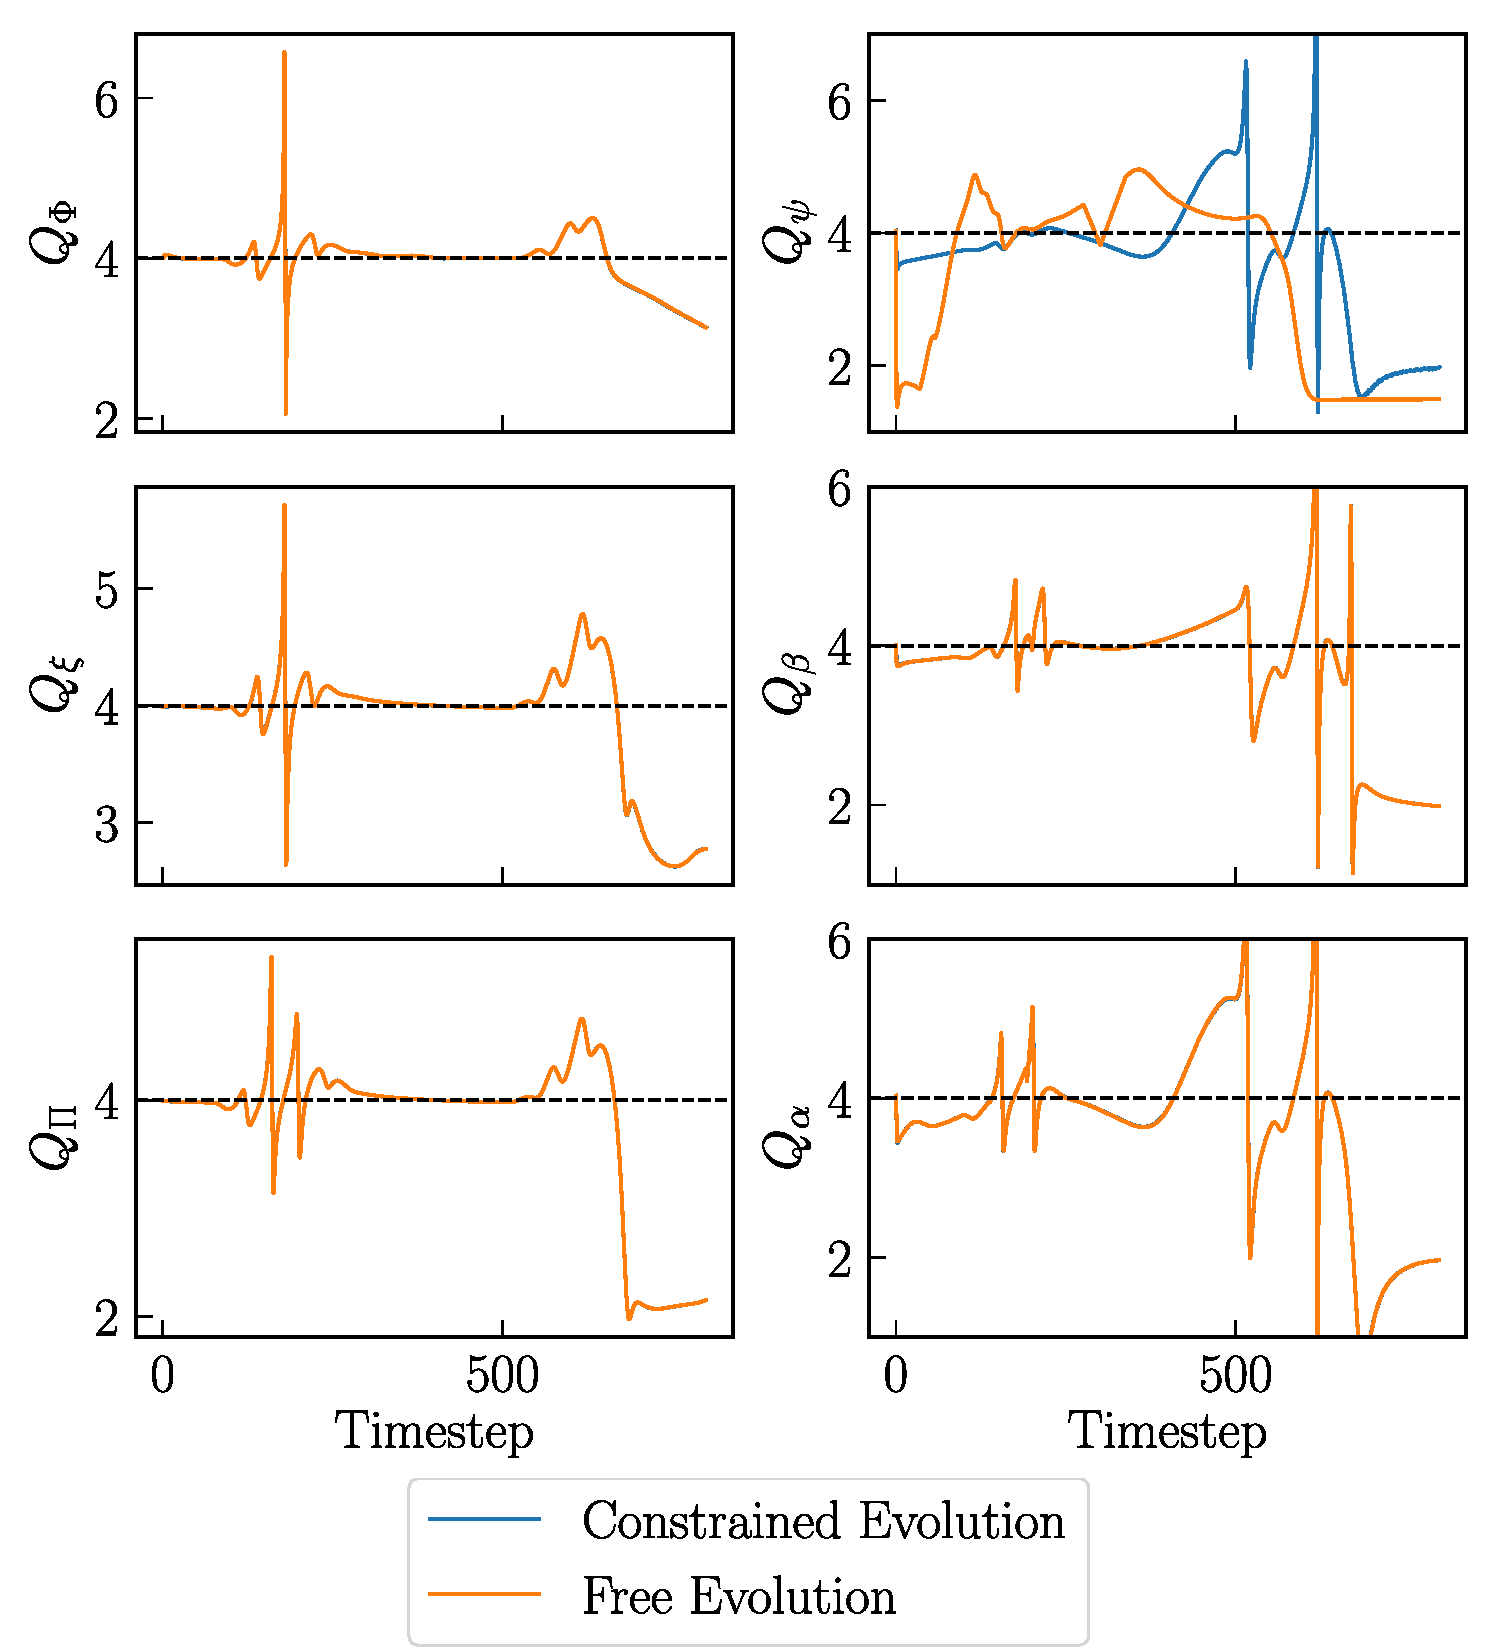
\includegraphics[width=\textwidth]{conv_plot.pdf}
	\caption{Convergence plot showing the quantity $Q_x$ for quantity $x$ at resolutions $N = 201, 401, 801$.  These resolutions are chosen such that $\Delta r = R_{max}/(N-1)$ is halved with each increased resolution.  The simulation was run with constrained evolution for $\psi$ (blue) and with free evolution for $\psi$ (orange), and both produce nearly identical second-order convergence plots except for $\psi$ itself.  All quantities converge at second order.  This simulation was run with $A = 0.01$, $\lambda = 0.5$, $\epsilon = 0.5$, $R_{max}=50$, $\Delta = 5$, $r_0 = 20$.}
\end{figure}


\section{Problem 6}
In this problem we are asked to write a function to locate apparent horizons if they form during a given simulation.  An apparent horizon is defined to be a location where the outward expansion of radially outgoing null vectors goes to zero -- namely, where outgoing light rays are unable to spread apart from each other because they cannot move outward to a location with greater surface area.  

The surface area of a given spatial sphere in spacetime is $A = 4 \pi R^2$, where $R = r \psi^2$ in our coordinates.  Thus an apparent horizon can be identified by computing where the fractional change in surface area, $\theta \equiv l^\nu (\partial_\nu A / A)$, goes to zero, where $l^\nu$ is an outward pointing null vector.  Using the derivative of the natural log function, we can rewrite this quantity as
\begin{equation} \label{eq:apparent_horiz_defn}
\begin{aligned}
\theta &\equiv \frac{l^\nu \partial_\nu A}{A} \\
&= l^\nu \partial_\nu \ln(A) \\
&= l^\nu \partial_\nu \ln(4 \pi R^2) \\
&= l^\nu \partial_\nu [\ln(4) + \ln(\pi) + 2 \ln(r)] \\
&= 2 l^\nu \partial_\nu \ln(R).
\end{aligned}
\end{equation}

Now we need to define $l^\nu$.  We want a vector that is null and outward-pointing in both the radial and time directions (because we're interested in the outward spread of null vectors in the positive radial and time directions).  We choose to define
\begin{equation}
l^\nu \equiv n^\nu + s^\nu,
\end{equation}
where $n^\nu$ is a purely timelike unit normal, and $s^\nu$ is a purely spacelike unit normal.  Both of these are relevant to the ADM decomposition used to derive the PDEs of the Einstein-KG system, so we have already computed $n^\nu$ and $n_\nu$ in the appendix for our coordinates (see equation \ref{eq:timelike_normal}).  Thus we can solve the equations
\begin{equation}
\begin{aligned}
s_\nu s^\nu &= 1 \\
n_\nu s^\nu &= 0
\end{aligned}
\end{equation}
to find the components of $s^\nu$.  Noting that the unit vector in the radial direction is $\partial_r$ in our coordinates, we can solve the above equations to find $s^\nu$:
\begin{equation}
\begin{aligned}
0 &= n_t s^t + n_r s^r + n_\theta s^\theta + n_\phi s^\phi \\
&= n_t s^t \\
&= -\alpha s^t \\
&= s^t,
\end{aligned}
\end{equation}
so the $t$ component is zero.  It is important to note that we have defined $s^\nu$ to be a radial vector, so $s^\theta = s^\phi = 0$.  Using the second equation we get:
\begin{equation}
\begin{aligned}
1 &= s_t s^t + s_r s^r \\
&= 0 + g_{rr} s^r s^r \\
&= \psi^4 s^r s^r, \\
\end{aligned}
\end{equation}
so inserting the unit vectors, we find that
\begin{equation}
s^\nu = (0, \psi^{-2} \partial_r, 0, 0).
\end{equation}

Now we can compute $\theta$ in our coordinates (suppressing the unit vectors):
\begin{equation}
\begin{aligned}
\theta &= 2 l^\nu \partial_\nu \ln(R) \\
&= 2 (n^\nu + s^\nu) \partial_\nu \ln(R) \\
&= 2 n^\nu \partial_\nu \ln(R) + 2 s^\nu \partial_\nu \ln(R) \\
&= 2 n^t \partial_t \ln(R) + 2 n^r \partial_r \ln(R) + 2 s^r \partial_r \ln(R) \\
&= 2 \alpha^{-1} \partial_t \ln(R) - 2 \alpha^{-1} \beta \partial_r \ln(R) + 2 \psi^{-2} \partial_r \ln(R); \\
\end{aligned}
\end{equation}
using Mathematica at this step to evaluate the derivatives (and using \ref{eq:psi_hyperbolic_eqn}), we get
\begin{equation}
\begin{aligned}
\theta &= \frac{2}{3 r \alpha \psi^3} [3 \alpha \psi - \beta \psi^3 + r \psi^3 \beta' + 6 r \alpha \psi'] \\
&= \frac{2}{3 r \alpha \psi^3} 3 \alpha \psi - \frac{2}{3 r \alpha \psi^3} \beta \psi^3 + \frac{2}{3 r \alpha \psi^3} r \psi^3 \beta' + \frac{2}{3 r \alpha \psi^3} 6 r \alpha \psi' \\
&= \frac{2}{r \psi^4} \Big( \psi^2 + 2 r \psi \psi' \Big) + \frac{2 r}{3 \alpha} \Big( - \frac{\beta}{r^2} + \frac{\beta'}{r} \Big), \\
\end{aligned}
\end{equation}
which may be rearranged to yield
\begin{equation}
\boxed{\theta = \frac{2}{r \psi^4} (r \psi^2)' + \frac{2 r}{3 \alpha} \Big( \frac{\beta}{r} \Big)' }
\end{equation}
which agrees with the project description.

\section{Problem 7}
We are now asked to compute the Ricci scalar in terms of the matter quantities (we compute it purely in terms of geometric quantities in the appendix).  We may do this quickly by noting that the full contraction of the Einstein equation with the metric yields
\begin{equation}
R = - 8 \pi T,
\end{equation}
where $T$ is the trace of the stress-energy tensor.  Computing the trace in Mathematica (see Mathematica notebook in GitHub repository) we get
\begin{equation}
T = \frac{\Pi^2 - \xi^2}{\psi^4},
\end{equation}
so
\begin{equation}
\boxed{ R = \frac{8 \pi (\xi^2 - \Pi^2)}{\psi^4} }
\end{equation}
which agrees with the project description.

\begin{thebibliography}{widestlabel}
	\bibitem{Pretorius06}
	F. Pretorius and M. W. Choptuik, ``Adaptive Mesh Refinement for Coupled Elliptic-Hyperbolic Systems", J. Comput. Phys. 218 (2006)
\end{thebibliography}

\appendix
\section{Derivation of the Governing PDEs}
It is possible to derive the equations in the handout starting from the ADM equations (taken from Shapiro and Baumgarte).  We may begin with some basic definitions before showing the full equations.  First we define the matter source terms
\begin{align}
\rho &= n_a n_b T^{ab} \\
S^i &= -\gamma^{ij} n^a T_{aj} \\
S_{ij} &= \gamma_{ia} \gamma_{jb} T^{ab} \\
S &= \gamma^{ij} S_{ij},
\end{align}
where $\gamma_{ij}$ is the spatial 3-metric, $n^a \equiv - g^{ab} \omega_b = -g^{ab} \alpha \nabla_b t$ is the unit normal to the spatial hyperslices, $T^{ab}$ is the stress-energy tensor, and $S_{ij}$ is the spatial stress-energy tensor.  It also helps to define the ADM line element
\begin{equation} \label{eq:ADM_line_element}
ds^2 = -\alpha^2 dt + \gamma_{ij} (dx^i + \beta^i dt) (dx^j + \beta^j dt)
\end{equation}
and the \textit{extrinsic curvature}
\begin{equation}
K_{ab} \equiv - \gamma_a^{~c} \gamma_b^{~d} \nabla_{(c} n_{d)} = - \gamma_a^{~c} \gamma_b^{~d} \nabla_c n_d.
\end{equation}
We'll also need the derivative operator
\begin{equation}
D_a f \equiv \gamma_{a}^{~b} \nabla_b f,
\end{equation}
for scalar $f$.

The ADM equations include: the \textit{Hamiltonian constraint}
\begin{equation}
R + K^2 - K_{ij} K^{ij} = 16 \pi \rho;
\end{equation}
the \textit{momentum constraint}
\begin{equation}
D_j (K^{ij} - \gamma^{ij} K) = 8 \pi S^{i};
\end{equation}
the \textit{evolution equation for the spatial metric}
\begin{equation} \label{eq:spatial_metric_evol}
\partial_t \gamma_{ij} = -2 \alpha K_{ij} + D_i \beta_j + D_j \beta_i;
\end{equation}
and the \textit{evolution equation for the extrinsic curvature}
\begin{equation}
\begin{aligned}
\partial_t K_{ij} &= \alpha (R_{ij} - 2 K_{ik} K^{k}_{~j} + K K_{ij}) - D_i D_j \alpha \\
&- 8 \pi \alpha (S_{ij} - \frac{1}{2} \gamma_{ij} (S - \rho)) + \beta^k \partial_k K_{ij} + K_{ik} \partial_j \beta^k + K_{kj} \partial_i \beta^k.
\end{aligned}
\end{equation}

Now let's use equation \ref{eq:ADM_line_element} to find the metric and inverse metric.  Reading off the metric, we have
\begin{equation}
g_{ab} =
\begin{pmatrix}
-\alpha^{2} + \beta_l \beta^l & \beta_i \\
\beta_j & \gamma_{ij}  \\
\end{pmatrix}
\end{equation}
and since $g_{\mu \lambda} g^{\lambda \nu} = \delta^\nu_\mu$, the inverse metric is (note: this differs in the off-diagonal terms from B\&S, but agrees with online lecture notes)
\begin{equation}
g^{ab} = 
\begin{pmatrix}
-\alpha^{-2} & \alpha^{-2} \beta^j \\
\alpha^{-2} \beta^i & \gamma^{ij} - \alpha^{-2} \beta^{i} \beta^{j} \\
\end{pmatrix}.
\end{equation}

We may now compute the unit normal to the spacelike hypersurfaces:
\begin{equation} \label{eq:timelike_normal}
\begin{aligned}
n^a &= -g^{ab} \alpha \nabla_b t \\
&= -g^{a t} \alpha \nabla_t t \\
&= (\alpha^{-1}, -\alpha^{-1} \beta^{a}),
\end{aligned}
\end{equation}
and similarly B\&S gives $n_a = (-\alpha, 0, 0, 0)$ because $n_a n^a = -1$ since $n^a$ is a timelike vector.

%\subsection{Applying Spherical Symmetry}
Now we assume the spherically symmetric spatial metric $\gamma_{ij} = \psi^4 \mathrm{diag}(1, r^2, r^2 \sin^2 \theta)$ in which $\beta^i = (\beta, 0, 0)$.  We can now use equation \ref{eq:spatial_metric_evol} to find the extrinsic curvature
\begin{equation}
\begin{aligned}
\partial_t \gamma_{ij} &= -2 \alpha K_{ij} + D_i \beta_j + D_j \beta_i \\
&= -2 \alpha K_{ij} + \gamma_{i}^{~l} \gamma_{j}^{~m} \nabla_l \beta_m + \gamma_j^{~m} \gamma_i^{~l} \nabla_m \beta_l \\
&= -2 \alpha K_{ij} + \gamma^{n l} \gamma_{i n} \gamma^{p m} \gamma_{j p} \nabla_l \beta_m + \gamma^{n m} \gamma_{j n} \gamma^{p l} \gamma_{i p} \nabla_m \beta_l \\
\partial_t \gamma_{r r} &= -2 \alpha K_{rr} + \gamma^{n l} \gamma_{r n} \gamma^{p m} \gamma_{r p} \nabla_l \beta_m + \gamma^{n m} \gamma_{r n} \gamma^{p l} \gamma_{r p} \nabla_m \beta_l \\
&= -2 \alpha K_{rr} + \gamma^{r r} \gamma_{r r} \gamma^{r r} \gamma_{r r} \nabla_r \beta_r + \gamma^{r r} \gamma_{r r} \gamma^{r r} \gamma_{r r} \nabla_r \beta_r \\
&= -2 \alpha K_{rr} + 2 \nabla_r \beta_r \\
&= -2 \alpha K_{rr} + 2 (\partial_r \beta_r - \Gamma^{\lambda}_{rr} \beta_\lambda) \\
&= -2 \alpha K_{rr} + 2 \Big[ \partial_r (\gamma_{rr} \beta^r) - \Gamma^{\lambda}_{rr} (\gamma_{\lambda q} \beta^{q}) \Big] \\
&= -2 \alpha K_{rr} + 2 \Big[ \partial_r (\gamma_{rr} \beta) - \Gamma^{r}_{rr} (\gamma_{r r} \beta) \Big] \\
&= -2 \alpha K_{rr} + 2 \Big[ 4 \psi^3 \psi' \beta + \psi^4 \beta' - (2\psi' \psi^{-1}) (\psi^4 \beta) \Big] \\
\partial_t (\psi^4) &= -2 \alpha K_{rr} + 4 \psi^3 \psi' \beta + 2 \psi^4 \beta' \\
K_{rr} &= \frac{1}{\alpha} \Big( 2 \psi^3 \psi' \beta + \psi^4 \beta' - 2 \psi^3 \dot{\psi} \Big) \\
\end{aligned}
\end{equation}
similarly
\begin{equation}
\begin{aligned}
\partial_t \gamma_{\theta \theta} &= -2 \alpha K_{\theta \theta} + D_\theta \beta_\theta + D_\theta \beta_\theta \\
r^2 4 \psi^3 \dot{\psi} &= -2 \alpha K_{\theta \theta} - 2 \Big( - \frac{2 \psi' r^2}{\psi} - r \Big) \gamma_{rr} \beta \\
\alpha K_{\theta \theta} &= 2 \psi' r^2 \psi^3 \beta + r \psi^4 \beta - 2 r^2 \psi^3 \dot{\psi}\\
K_{\theta \theta} &= \frac{1}{\alpha} \Big( 2 \psi' r^2 \psi^3 \beta + r \psi^4 \beta - 2 r^2 \psi^3 \dot{\psi} \Big), \\
\end{aligned}
\end{equation}
and
\begin{equation}
\begin{aligned}
\partial_t \gamma_{\phi \phi} &= -2 \alpha K_{\phi \phi} + D_\phi \beta_\phi + D_\phi \beta_\phi \\
\partial_t (\psi^4 r^2 \sin^2 \theta) &= -2 \alpha K_{\phi \phi} + 2 (\partial_\phi \beta_\phi - \Gamma^{\lambda}_{\phi \phi} \beta_\lambda) \\
r^2 \sin^2 \theta (4 \psi^3 \dot{\psi}) &= -2 \alpha K_{\phi \phi} + 2 (0 - \Gamma^{r}_{\phi \phi} \beta_r) \\
\alpha K_{\phi \phi} &= \Big( \frac{2 \psi' r^2}{\psi} + r \Big) \sin^2 \theta ( \gamma_{rr} \beta) - 2 r^2 \psi^3 \dot{\psi} \sin^2 \theta \\
K_{\phi \phi} &= \frac{1}{\alpha} \Big( 2 \psi' r^2 \psi^3 \beta + r \psi^4 \beta - 2 r^2 \psi^3 \dot{\psi} \Big) \sin^2 \theta \\
&= K_{\theta \theta} \sin^2 \theta
\end{aligned}
\end{equation}
We also need the trace of the extrinsic curvature:
\begin{equation}
\begin{aligned}
K &= \gamma^{ij} K_{ij} \\
&= \gamma^{rr} K_{rr} + \gamma^{\theta \theta} K_{\theta \theta} + \gamma^{\phi \phi} K_{\phi \phi} \\
&= \psi^{-4} K_{rr} + \psi^{-4} r^{-2} K_{\theta \theta} + \psi^{-4} r^{-2} \sin^{-2} \theta K_{\phi \phi} \\
&= \psi^{-4} \frac{1}{\alpha} \Big( 2 \psi^3 \psi' \beta + \psi^4 \beta' - 2 \psi^3 \dot{\psi} \Big) + \psi^{-4} r^{-2} \frac{1}{\alpha} \Big( 2 \psi' r^2 \psi^3 \beta + r \psi^4 \beta - 2 r^2 \psi^3 \dot{\psi} \Big) \\
&+ \psi^{-4} r^{-2} \sin^{-2} \theta \frac{1}{\alpha} \Big( 2 \psi' r^2 \psi^3 \beta + r \psi^4 \beta - 2 r^2 \psi^3 \dot{\psi} \Big) \sin^2 \theta \\
&= \frac{6 \psi' \beta}{\psi \alpha} + \frac{\beta'}{\alpha} - \frac{6 \dot{\psi}}{\psi \alpha} + \frac{2 \beta}{r \alpha} \\
%&= \psi^{-4} \frac{1}{\alpha} \Big( 2 \psi^3 \psi' \beta + \psi^4 \beta' - 2 \psi^3 \dot{\psi} \Big)  - \psi^{-4} r^{-2} \frac{2 r^2 \psi^3 \dot{\psi}}{\alpha} \\
%&- \psi^{-4} r^{-2} \sin^{-2} \theta \frac{2 r^2 \sin^2 \theta \psi^3 \dot{\psi}}{\alpha} \\
%&= \frac{2 \psi' \beta}{\psi \alpha} + \frac{\beta'}{\alpha} - \frac{6 \dot{\psi}}{\psi \alpha}. \\
\end{aligned}
\end{equation}
%We can compute a straightforward sanity check using a common contraction of one of the ADM equations which also yields the trace of the extrinsic curvature (note below $\gamma = \mathrm{det}[\gamma_{ij}]$):
%\begin{equation}
%\begin{aligned}
%\partial_t \ln(\gamma^{1/2}) &= -\alpha K + D_i \beta^i \\
%\partial_t \ln( [\psi^4 \psi^4 r^2 \psi^4 r^2 \sin^2 \theta]^{1/2} ) &= -\alpha K + D_i \beta^i \\
%\partial_t \ln( \psi^6 r^2 \sin \theta ) &= -\alpha K + D_i \beta^i \\
%\frac{6 \psi^5 \dot{\psi} r^2 \sin^2 \theta}{\psi^6 r^2 \sin^2 \theta} &= -\alpha K + D_i \beta^i \\
%\frac{6 \dot{\psi}}{\psi} &= -\alpha K + D_r (\beta^r) \\
%&= -\alpha K + \gamma_r^{~b} \nabla_b (\beta^r) \\
%&= -\alpha K + \gamma^{a b} \gamma_{r a} \nabla_b (\beta^r) \\
%&= -\alpha K + \gamma^{r r} \gamma_{r r} \nabla_r (\beta^r) \\
%&= -\alpha K + \gamma^{r r} \gamma_{r r} (\partial_r \beta^r + \Gamma_{r \lambda}^{r} \beta^\lambda) \\
%&= -\alpha K + \beta' + \frac{2 \psi'}{\psi} \beta \\
%-\alpha K &= \frac{6 \dot{\psi}}{\psi} - \beta' - \frac{2 \psi'}{\psi} \beta \\
%K &= \frac{\beta'}{\alpha} + \frac{2 \beta \psi'}{\psi \alpha} -\frac{6 \dot{\psi}}{\psi \alpha}, \\
%\end{aligned}
%\end{equation}
%which agrees with our result above.

Now we can compute the Ricci tensor.  In the ADM formalism Christoffel symbols with upper index zero are equal to zero, resulting in the equation
\begin{equation}
R_{ij} = \partial_k \Gamma^k_{ij} - \partial_j \Gamma^k_{ik} + \Gamma^k_{ij} \Gamma^l_{kl} - \Gamma^k_{il} \Gamma^l_{jk},
\end{equation}
where the Christoffel symbols are
\begin{equation}
\Gamma^i_{jk} = \frac{1}{2} \gamma^{il} (\partial_k \gamma_{lj} + \partial_j \gamma_{lk} - \partial_l \gamma_{jk}).
\end{equation}

For our spatial metric the surviving connection coefficients with an $r$ upper index are:
\begin{equation}
\begin{aligned}
\Gamma^{r}_{rr} &= \frac{1}{2} \gamma^{rl} (\partial_r \gamma_{lr} + \partial_r \gamma_{lr} - \partial_l \gamma_{rr})\\
&= \frac{1}{2} \gamma^{rr} (\partial_r \gamma_{rr} + \partial_r \gamma_{rr} - \partial_r \gamma_{rr})\\
&= \frac{1}{2} \gamma^{rr} (\partial_r \gamma_{rr})\\
&= \frac{1}{2} \psi^{-4} (\partial_r \psi^4)\\
&= \frac{1}{2} \psi^{-4} (4 \psi^3 \psi')\\
&= \frac{2 \psi'}{\psi} \\
\Gamma^r_{\theta \theta} &= \frac{1}{2} \gamma^{r r} (- \partial_r \gamma_{\theta \theta}) \\
&= \frac{1}{2 \psi^4} (- \partial_r \psi^4 r^2 ) \\
&= \frac{1}{2 \psi^4} (- 4 \psi^3 \psi' r^2 - 2 \psi^4 r ) \\
&= - \frac{2 \psi' r^2}{\psi} - r \\
\Gamma^r_{\phi \phi} &= \frac{1}{2} \gamma^{r r} ( - \partial_r \gamma_{\phi \phi}) \\
&= \frac{1}{2 \psi^4} ( - \partial_r \psi^4 r^2 \sin^2 \theta) \\
&= \frac{1}{2 \psi^4} ( - 4 \psi^3 \psi' r^2 - 2 \psi^4 r ) \sin^2 \theta \\
&= - \Big( \frac{2 \psi' r^2}{\psi} + r \Big) \sin^2 \theta, \\
\end{aligned}
\end{equation}
those with a $\theta$ upper index are:
\begin{equation}
\begin{aligned}
\Gamma^{\theta}_{r \theta} &= \frac{1}{2} \gamma^{\theta \theta} (\partial_r \gamma_{\theta \theta}) \\
&= \frac{1}{2} \frac{1}{\psi^4 r^2} (\partial_r \psi^4 r^2) \\
&= \frac{1}{2} \frac{1}{\psi^4 r^2} (4 \psi^3 \psi' r^2 + 2 \psi^4 r) \\
&= \frac{2 \psi'}{\psi}  + \frac{1}{r} \\
\Gamma^\theta_{\phi \phi} &= \frac{1}{2} \gamma^{\theta \theta} (\partial_\phi \gamma_{\theta \phi} + \partial_\phi \gamma_{\theta \phi} - \partial_\theta \gamma_{\phi \phi}) \\
&= - \frac{1}{2} \psi^{-4} r^{-2} \partial_\theta (\psi^4 r^2 \sin^2 \theta) \\
&= - \sin \theta \cos \theta \\
\end{aligned}
\end{equation}
and the ones with a $\phi$ upper index are
\begin{equation}
\begin{aligned}
\Gamma^{\phi}_{r \phi} &= \frac{1}{2} \gamma^{\phi \phi} (\partial_r \gamma_{\phi \phi}) \\
&= \frac{1}{2} \frac{1}{\psi^4 r^2 \sin^2 \theta} (\partial_r \psi^4 r^2 \sin^2 \theta) \\
&= \frac{1}{2} \frac{1}{\psi^4 r^2} (4 \psi^3 \psi' r^2 + 2 \psi^4 r) \\
&= \frac{2 \psi'}{\psi} + \frac{1}{r} \\
\Gamma^{\phi}_{\phi \theta} &= \frac{1}{2} \gamma^{\phi l} (\partial_\theta \gamma_{l \phi} + \partial_\phi \gamma_{l \theta} - \partial_l \gamma_{\phi \theta}) \\
&= \frac{1}{2} \gamma^{\phi \phi} (\partial_\theta \gamma_{\phi \phi}) \\
&= \cot \theta \\
\end{aligned}
\end{equation}
and the Christoffel symbols are symmetric in their lower indices, so permuting them results in a symbol with the same value.

The Ricci tensor is
\begin{equation}
R_{ij} = \partial_k \Gamma^k_{ij} - \partial_j \Gamma^k_{ik} + \Gamma^k_{ij} \Gamma^l_{kl} - \Gamma^k_{il} \Gamma^l_{jk},
\end{equation}
so
\begin{equation}
\begin{aligned}
R_{rr} &= \partial_k \Gamma^k_{rr} - \partial_r \Gamma^k_{rk} + \Gamma^k_{rr} \Gamma^l_{kl} - \Gamma^k_{rl} \Gamma^l_{rk} \\
&= \partial_r \Gamma^r_{rr} - \partial_r \Gamma^r_{r r} - \partial_r \Gamma^\theta_{r\theta} - \partial_r \Gamma^\phi_{r\phi} + \Gamma^r_{rr} \Gamma^r_{rr} + \Gamma^r_{rr} \Gamma^\theta_{r\theta} + \Gamma^r_{rr} \Gamma^\phi_{r \phi} - \Gamma^\theta_{r\theta} \Gamma^\theta_{r\theta} - \Gamma^\phi_{r \phi} \Gamma^\phi_{r\phi} - \Gamma^r_{rr} \Gamma^r_{rr} \\
&= - 2 \partial_r \Gamma^\theta_{r\theta} + 2 \Gamma^r_{rr} \Gamma^\theta_{r\theta} - 2 \Gamma^\theta_{r\theta} \Gamma^\theta_{r\theta} \\
&= - 2 \partial_r \Big( \frac{2 \psi'}{\psi}  + \frac{1}{r} \Big) + 2 \frac{2 \psi'}{\psi} \Big( \frac{2 \psi'}{\psi}  + \frac{1}{r} \Big) - 2 \Big( \frac{2 \psi'}{\psi}  + \frac{1}{r} \Big)^2 \\
&= - \frac{4 \psi''}{\psi} + \frac{4 \psi'^2}{\psi^2} + \frac{2}{r^2} + \frac{8 \psi'^2}{\psi^2}  + \frac{4 \psi'}{r \psi} - \frac{8 \psi'^2}{\psi^2} - \frac{8 \psi'}{r \psi} - \frac{2}{r^2} \\
&= - \frac{4 \psi''}{\psi} + \frac{4 \psi'^2}{\psi^2} - \frac{4 \psi'}{r \psi},
\end{aligned}
\end{equation}
which agrees with the UBC handout.  Similarly
\begin{equation}
\begin{aligned}
R_{\theta \theta} &= \partial_k \Gamma^k_{\theta \theta} - \partial_\theta \Gamma^k_{\theta k} + \Gamma^k_{\theta \theta} \Gamma^l_{kl} - \Gamma^k_{\theta l} \Gamma^l_{\theta k} \\
&= \partial_r \Gamma^r_{\theta \theta} - \partial_\theta \Gamma^\phi_{\theta \phi} + \Gamma^r_{\theta \theta} \Gamma^r_{rr} + \Gamma^r_{\theta \theta} \Gamma^\theta_{r\theta} + \Gamma^r_{\theta \theta} \Gamma^\phi_{r\phi} - \Gamma^r_{\theta \theta} \Gamma^\theta_{\theta r} - \Gamma^\theta_{\theta r} \Gamma^r_{\theta \theta} - \Gamma^\phi_{\theta \phi} \Gamma^\phi_{\theta \phi} \\
&= \partial_r \Gamma^r_{\theta \theta} - \partial_\theta \Gamma^\phi_{\theta \phi} + \Gamma^r_{\theta \theta} \Gamma^r_{rr} + 2 \Gamma^r_{\theta \theta} \Gamma^\theta_{r\theta} - 2 \Gamma^r_{\theta \theta} \Gamma^\theta_{\theta r} - \Gamma^\phi_{\theta \phi} \Gamma^\phi_{\theta \phi} \\
&= \partial_r \Big( - \frac{2 \psi' r^2}{\psi} - r \Big) - \partial_\theta \cot \theta + \Big( - \frac{2 \psi' r^2}{\psi} - r \Big) \frac{2 \psi'}{\psi} \\
&+ 2 \Big( - \frac{2 \psi' r^2}{\psi} - r \Big) \Big( \frac{2 \psi'}{\psi}  + \frac{1}{r} \Big) - 2 \Big( - \frac{2 \psi' r^2}{\psi} - r \Big) \Big( \frac{2 \psi'}{\psi}  + \frac{1}{r} \Big) - \cot \theta \cot \theta \\
&=  - \frac{2 \psi'' r^2}{\psi} - \frac{4 \psi' r}{\psi} + \frac{2 \psi'^2 r^2}{\psi^2} - 1 + \csc^2 \theta - \frac{4 \psi'^2 r^2}{\psi^2} - \frac{2 r \psi'}{\psi} - \cot^2 \theta \\
&=  - \frac{2 \psi'' r^2}{\psi} - \frac{6 \psi' r}{\psi} - \frac{2 \psi'^2 r^2}{\psi^2}, \\
\end{aligned}
\end{equation}
which agrees with the UBC handout.  Finally we have
\begin{equation}
\begin{aligned}
R_{\phi \phi} &= \partial_k \Gamma^k_{\phi \phi} - \partial_\phi \Gamma^k_{\phi k} + \Gamma^k_{\phi \phi} \Gamma^l_{kl} - \Gamma^k_{\phi l} \Gamma^l_{\phi k} \\
&= \partial_r \Gamma^r_{\phi \phi} + \partial_\theta \Gamma^\theta_{\phi \phi} + \Gamma^r_{\phi \phi} \Gamma^\theta_{r\theta} + \Gamma^r_{\phi \phi} \Gamma^\phi_{r\phi} + \Gamma^r_{\phi \phi} \Gamma^r_{r r} + \Gamma^\theta_{\phi \phi} \Gamma^\phi_{\theta \phi} \\
&- \Gamma^r_{\phi \phi} \Gamma^\phi_{\phi r} - \Gamma^\phi_{\phi \theta} \Gamma^\theta_{\phi \phi} - \Gamma^\theta_{\phi \phi} \Gamma^\phi_{\phi \theta} - \Gamma^\phi_{\phi r} \Gamma^{r}_{\phi \phi} \\
&= \partial_r \Gamma^r_{\phi \phi} + \partial_\theta \Gamma^\theta_{\phi \phi} + \Gamma^r_{\phi \phi} \Gamma^r_{r r} - \Gamma^\theta_{\phi \phi} \Gamma^\phi_{\phi \theta} \\
&= - \sin^2 \theta \partial_r \Big( \frac{2 \psi' r^2}{\psi} + r \Big) - \partial_\theta (\sin \theta \cos \theta) - \Big( \frac{2 \psi' r^2}{\psi} + r \Big) \sin^2 \theta \frac{2 \psi'}{\psi} + \cos^2 \theta \\
&= - \frac{2 \psi'' r^2}{\psi} \sin^2 \theta - \frac{4 \psi' r}{\psi} \sin^2 \theta + \frac{2 \psi'^2 r^2}{\psi^2} \sin^2 \theta - \frac{4 \psi'^2 r^2}{\psi^2} \sin^2 \theta - \frac{2 r \psi'}{\psi} \sin^2 \theta \\
&= - \frac{2 \psi'' r^2}{\psi} \sin^2 \theta - \frac{6 \psi' r}{\psi} \sin^2 \theta - \frac{2 \psi'^2 r^2}{\psi^2} \sin^2 \theta \\
&= R_{\theta \theta} \sin^2 \theta,
\end{aligned}
\end{equation}
which also agrees with the UBC handout.

We can now compute the Ricci scalar
\begin{equation}
\begin{aligned}
R &= \gamma^{r r} R_{r r} + \gamma^{\theta \theta} R_{\theta \theta} + \gamma^{\phi \phi} R_{\phi \phi} \\
&= \psi^{-4} R_{rr} + \psi^{-4} r^{-2} R_{\theta \theta} + \psi^{-4} r^{-2} \sin^{-2} \theta R_{\theta \theta} \sin^2 \theta \\
&= \psi^{-4} R_{rr} + 2 \psi^{-4} r^{-2} R_{\theta \theta} \\
&= - \frac{4 \psi''}{\psi^5} + \frac{4 \psi'^2}{\psi^6} - \frac{4 \psi'}{r \psi^5} - \frac{4 \psi''}{\psi^5} - \frac{12 \psi'}{r \psi^5} - \frac{4 \psi'^2}{\psi^6} \\
&= - \frac{8 \psi''}{\psi^5} - \frac{16 \psi'}{r \psi^5}, \\
\end{aligned}
\end{equation}
which again agrees with the UBC handout.

\subsection{Matter Sources}
Now we can compute the matter source quantities.  Before we begin, we first need to find the stress-energy tensor for the scalar field, $T^{ab}$.  We may derive it beginning with the well-known Lagrangian of a massless scalar field $\Phi$:
\begin{equation}
\Lagr = \frac{1}{2} g^{\mu \nu} \partial_\mu \Phi \partial_\nu \Phi,
\end{equation}
so
\begin{equation}
\begin{aligned}
T^{\mu}_{~\nu} &\equiv \frac{\partial \Lagr}{\partial (\partial_\mu \Phi)} \partial_\nu \Phi - \delta^\mu_\nu \Lagr \\
T^{\mu \nu} &= g^{\gamma \nu} \frac{\partial \Lagr}{\partial (\partial_\mu \Phi)} \partial_\gamma \Phi - g^{\gamma \nu} \delta^\mu_\gamma \Lagr \\
&= g^{\gamma \nu} \Big( \frac{1}{2} g^{\mu \nu} \delta^\mu_\nu \partial_\nu \Phi + \frac{1}{2} g^{\mu \nu} \partial_\mu \Phi \delta^\mu_\mu \Big) \partial_\gamma \Phi	 - g^{\gamma \nu} \delta^\mu_\gamma \frac{1}{2} g^{\mu \nu} \partial_\mu \Phi \partial_\nu \Phi \\
&= g^{\gamma \nu} \Big( \frac{1}{2} \partial^\mu \Phi + \frac{1}{2} \partial^\nu \Phi \Big) \partial_\gamma \Phi - g^{\gamma \nu} \delta^\mu_\gamma \frac{1}{2} g^{\mu \nu} \partial_\mu \Phi \partial_\nu \Phi \\
&= \partial^\mu \Phi \partial^\nu \Phi - \frac{1}{2} g^{\mu \nu} \partial^\gamma \Phi \partial_\gamma \Phi, \\
\end{aligned}
\end{equation}
which agrees with the project description, equation 3.

Now we can compute $\rho$:
\begin{equation}
\begin{aligned}
\rho &= n_a n_b T^{ab} \\
&= n_t n_t T^{tt} + n_r n_r T^{rr} + n_\theta n_\theta T^{\theta \theta} + n_\phi n_\phi T^{\phi \phi} \\
&= \alpha^{2} T^{tt} \\
&= \alpha^{2} \Big( \partial^t \Phi \partial^t \Phi - \frac{1}{2} g^{t t} \partial^\gamma \Phi \partial_\gamma \Phi \Big) \\
&= \alpha^{2} \Big( g^{\lambda t} g^{\rho t} \partial_\lambda \Phi \partial_\rho \Phi - \frac{1}{2} g^{t t} g^{\mu \nu} \partial_{\mu} \Phi \partial_{\nu} \Phi \Big) \\
&= \alpha^{2} \Big( g^{t t} g^{t t} \partial_t \Phi \partial_t \Phi + 2 g^{r t} g^{t t} \partial_r \Phi \partial_t \Phi + g^{r t} g^{r t} \partial_r \Phi \partial_r \Phi \\
&- \frac{1}{2} g^{t t} g^{t t} \partial_{t} \Phi \partial_{t} \Phi - g^{t t} g^{t r} \partial_{t} \Phi \partial_{r} \Phi - \frac{1}{2} g^{t t} g^{r r} \partial_{r} \Phi \partial_{r} \Phi \Big) \\
&= \alpha^{2} \Big( \frac{1}{2} g^{t t} g^{t t} \partial_t \Phi \partial_t \Phi + g^{r t} g^{t t} \partial_r \Phi \partial_t \Phi + g^{r t} g^{r t} \partial_r \Phi \partial_r \Phi - \frac{1}{2} g^{t t} g^{r r} \partial_{r} \Phi \partial_{r} \Phi \Big) \\
&= \alpha^{2} \Big( \frac{1}{2} (-\alpha^{-2}) (-\alpha^{-2}) \dot{\Phi}^2 + (\alpha^{-2} \beta) (-\alpha^{-2}) \Phi' \dot{\Phi} \\
&+ (\alpha^{-2} \beta) (\alpha^{-2} \beta) \Phi'^2 - \frac{1}{2} (-\alpha^{-2}) (\gamma^{rr} - \alpha^{-2} \beta^2) \Phi'^2 \Big) \\
&= \frac{1}{2} \alpha^{-2} \dot{\Phi}^2 - \beta \alpha^{-2} \Phi' \dot{\Phi} + \alpha^{-2} \beta^2 \Phi'^2 + \frac{1}{2} (\psi^{-4} - \alpha^{-2} \beta^2) \Phi'^2 \\
&= \frac{1}{2} \alpha^{-2} \dot{\Phi}^2 - \beta \alpha^{-2} \Phi' \dot{\Phi} + \frac{1}{2} \alpha^{-2} \beta^2 \Phi'^2 + \frac{1}{2} \psi^{-4} \Phi'^2 \\
&= \frac{1}{2 \psi^{4}} \Big( \Pi^2 + \xi^2 \Big) \\
\end{aligned}
\end{equation}

Now we can do $S_{ij}$:
\begin{equation}
\begin{aligned}
S_{rr} &= \gamma_{ra} \gamma_{rb} T^{ab} \\
&= \gamma_{rr} \gamma_{rr} T^{rr} + \gamma_{r \theta} \gamma_{r\theta} T^{\theta \theta} + \gamma_{r\phi} \gamma_{r\phi} T^{\phi \phi} \\
&= (\psi^4) (\psi^4) T^{rr} \\
&= \psi^8 \Big( g^{rr} g^{rr} \partial_r \Phi \partial_r \Phi - \frac{1}{2} g^{r r} g^{\mu \nu} \partial_\mu \Phi \partial_\nu \Phi \Big) \\
&= \psi^8 \Big( \psi^{-8} \Phi'^2 - \frac{1}{2} \psi^{-4} g^{t t} \dot{\Phi}^2 - \frac{1}{2} 2 \psi^{-4} g^{t r} \dot{\Phi} \Phi' - \frac{1}{2} \psi^{-4} g^{r r} \Phi'^2 \Big) \\
&= \frac{1}{2} \Phi'^2 + \frac{1}{2} \psi^4 \alpha^{-2} \Big( \dot{\Phi}^2 - 2 \beta \dot{\Phi} \Phi' + \beta^2 \Phi'^2 \Big) \\
&= \frac{1}{2} \xi^2 + \frac{1}{2} \psi^4 \alpha^{-2} \frac{\alpha^2}{\psi^4} \Pi^2 \\
&= \frac{1}{2} \xi^2 + \frac{1}{2} \Pi^2 \\
\end{aligned}
\end{equation}
and
\begin{equation}
\begin{aligned}
S_{\theta \theta} &= \gamma_{\theta a} \gamma_{\theta b} T^{ab} \\
&= \gamma_{\theta \theta} \gamma_{\theta \theta} T^{\theta \theta} \\
&= (\psi^4 r^2) (\psi^4 r^2) T^{\theta \theta} \\
&= (\psi^8 r^4) \Big( \partial^\theta \Phi \partial^\theta \Phi - \frac{1}{2} g^{\theta \theta} g^{\mu \nu} \partial_\mu \Phi \partial_\nu \Phi  \Big) \\
&= - \frac{1}{2} (\psi^8 r^4) \Big( g^{\theta \theta} g^{t t} \dot{\Phi}^2 + 2 g^{\theta \theta} g^{t r} \dot{\Phi} \Phi' + g^{\theta \theta} g^{r r} \Phi'^2  \Big) \\
&= - \frac{1}{2} \Big( - \psi^4 r^2 \alpha^{-2} \dot{\Phi}^2 + 2 \psi^4 r^2 \alpha^{-2} \beta \dot{\Phi} \Phi' + \psi^4 r^2 \psi^{-4} \Phi'^2 - \psi^4 r^2 \alpha^{-2} \beta^2 \Phi'^2 \Big) \\
&= - \frac{1}{2} r^2 \Big( - \psi^4 \alpha^{-2} (\dot{\Phi}^2 - 2 \beta \dot{\Phi} \xi + \beta^2 \xi^2) + \xi^2 \Big) \\
&= \frac{r^2}{2} \Big( \Pi^2 - \xi^2 \Big) \\
\end{aligned}
\end{equation}
and
\begin{equation}
\begin{aligned}
S_{\phi \phi} &= \gamma_{\phi a} \gamma_{\phi b} T^{ab} \\
&= \gamma_{\phi \phi} \gamma_{\phi \phi} T^{\phi \phi} \\
&= (\psi^4 r^2 \sin^2 \theta) (\psi^4 r^2 \sin^2 \theta) \Big( \partial^\phi \Phi \partial^\phi \Phi - \frac{1}{2} g^{\phi \phi} \partial^\gamma \Phi \partial_\gamma \Phi  \Big) \\
&= - (\psi^4 r^2 \sin^2 \theta) \Big( \frac{1}{2} g^{t t} \partial_t \Phi \partial_t \Phi + \frac{1}{2} 2 g^{t r} \partial_t \Phi \partial_r \Phi + \frac{1}{2} g^{r r} \partial_r \Phi \partial_r \Phi \Big) \\
&= - \frac{1}{2} (\psi^4 r^2 \sin^2 \theta) \Big( -\alpha^{-2} \dot{\Phi}^2 + 2 \alpha^{-2} \beta \dot{\Phi} \xi - \alpha^{-2} \beta^2 \xi^2 + \psi^{-4} \xi^2 \Big) \\
&= \frac{r^2 \sin^2 \theta}{2} \Big( \Pi^2 - \xi^2 \Big). \\
\end{aligned}
\end{equation}
We will need the trace of this tensor
\begin{equation}
\begin{aligned}
S &= \gamma^{rr} S_{rr} + \gamma^{\theta \theta} S_{\theta \theta} + \gamma^{\phi \phi} S_{\phi \phi} \\
&= \psi^{-4} \frac{1}{2} \Big( \xi^2 + \Pi^2 \Big) + \psi^{-4} \frac{1}{2} \Big( \Pi^2 - \xi^2 \Big) + \psi^{-4} \frac{1}{2} \Big( \Pi^2 - \xi^2 \Big) \\
&= \frac{1}{2 \psi^{4}} ( 3 \Pi^2 - \xi^2). \\
\end{aligned}
\end{equation}

We will also need the quantity
\begin{equation}
\begin{aligned}
S^i &= - \gamma^{ij} n^a T_{aj} \\
S^r &= - \gamma^{rr} n^a T_{a r} \\
&= - \gamma^{rr} n^t T_{t r} - \gamma^{rr} n^r T_{r r} \\
&= - \psi^{-4} \alpha^{-1} g_{t \mu} g_{\nu r} T^{\mu \nu} + \psi^{-4} \alpha^{-1} \beta g_{r \mu} g_{\nu r} T^{\mu \nu} \\
&= - \psi^{-4} \alpha^{-1} (g_{t t} g_{t r} T^{t t} + g_{t t} g_{r r} T^{t r} + g_{t r} g_{t r} T^{r t} + g_{t r} g_{r r} T^{r r}) \\
&+ \psi^{-4} \alpha^{-1} \beta (g_{r t} g_{t r} T^{t t} + g_{r t} g_{r r} T^{t r} + g_{r r} g_{t r} T^{r t} + g_{r r} g_{r r} T^{r r}); \\
\end{aligned}
\end{equation}
using Mathematica we find
\begin{equation}
\begin{aligned}
S^r &= \frac{\Phi' (-\dot{\Phi} + \beta \Phi')}{\alpha \psi^4} \\
&= - \frac{\xi (\dot{\Phi} - \beta \xi)}{\alpha \psi^4} \\
&= - \frac{\xi \Pi}{\psi^6}. \\
\end{aligned}
\end{equation}
Similarly,
\begin{equation}
\begin{aligned}
S^\theta &= - \gamma^{\theta \theta} n^t T_{t \theta} - \gamma^{\theta \theta} n^r T_{r \theta} \\
&= - \gamma^{\theta \theta} \alpha^{-1} g_{tt} g_{t \mu} g_{\nu \theta} T^{\mu \nu} + \gamma^{\theta \theta} \alpha^{-1} \beta g_{r \mu} g_{\nu \theta} T^{\mu \nu} \\
&= - \gamma^{\theta \theta} \alpha^{-1} g_{tt} (g_{t t} g_{t \theta} T^{t t} + g_{t t} g_{r \theta} T^{t r} + g_{t t} g_{\theta \theta} T^{t \theta} + g_{t r} g_{\nu t} T^{r t} \\
&+ g_{t r} g_{r \theta} T^{r r} + g_{t r} g_{\theta \theta} T^{r \theta} + g_{t \theta} g_{t \theta} T^{\theta t} + g_{t \theta} g_{r r} T^{\theta r} + g_{t \theta} g_{\theta \theta} T^{\theta \theta}) \\
&+ \gamma^{\theta \theta} \alpha^{-1} \beta (g_{r t} g_{t \theta} T^{t t} + g_{r t} g_{r \theta} T^{t r} + g_{r t} g_{\theta \theta} T^{t \theta} + g_{r r} g_{t \theta} T^{r t} \\
&+ g_{r r} g_{r \theta} T^{r r} + g_{r r} g_{\theta \theta} T^{r \theta} + g_{r \theta} g_{t \theta} T^{\theta t} + g_{r \theta} g_{r \theta} T^{\theta r} + g_{r \theta} g_{\theta \theta} T^{\theta \theta}) \\
&= 0
\end{aligned}
\end{equation}
and likewise
\begin{equation}
S^\phi = 0.
\end{equation}

\subsection{Checking the $\psi$ Hyperbolic Equation}
Now we can begin checking equations.  We are told that using our remaining coordinate freedom to choose \textit{maximal slicing} results in the equation $K = 0$, so
\begin{equation}
\begin{aligned}
0 &= \frac{6 \psi' \beta}{\psi \alpha} + \frac{\beta'}{\alpha} - \frac{6 \dot{\psi}}{\psi \alpha} + \frac{2 \beta}{r \alpha} \\
6 \dot{\psi} &= 6 \psi' \beta + \beta' \psi + \frac{2 \beta \psi}{r} \\
\dot{\psi} &= \psi' \beta + \frac{\beta' \psi}{6} + \frac{\beta \psi}{3 r}; \\
\end{aligned}
\end{equation}
rearranging once more gives
\begin{equation}
\boxed{\dot{\psi} = \beta \Big(\psi' + \frac{\psi}{3 r} \Big) + \frac{\beta' \psi}{6} }
\end{equation}
which agrees with the project handout.

\subsection{Checking the $\alpha$ Constraint Equation}
Beginning with a contraction of the evolution equation for the extrinsic curvature (B \& S equation 2.137) and applying the maximal slicing condition ($K = 0$) we begin with
\begin{equation}
0 = - \gamma^{ij} D_i D_j \alpha + \alpha (K_{ij} K^{ij} + 4 \pi (\rho + S));
\end{equation}
evaluation of the first term on the right-hand side is subtle, so we'll do it explicitly:
\begin{equation}
\begin{aligned}
\gamma^{ij} D_i D_j \alpha &= \gamma^{ij} \gamma_{i}^{~a} \nabla_a (\gamma_{j}^{~b} \nabla_b \alpha) \\
&= \gamma^{ij} \gamma_{i}^{~a} \nabla_a (\gamma_{j}^{~b} \nabla_b \alpha) \\
&= \gamma^{ij} \gamma_{i}^{~a} \Big[ \partial_a (\gamma_{j}^{~b} \nabla_b \alpha) - \Gamma^{\lambda}_{a j} (\gamma_{\lambda}^{~b} \nabla_b \alpha) \Big] \\
&= \gamma^{rr} \gamma_{r}^{~r} \Big[ \partial_r (\gamma_{r}^{~r} \nabla_r \alpha) - \Gamma^{r}_{r r} (\gamma_{r}^{~r} \nabla_r \alpha) \Big] \\
&+ \gamma^{\theta \theta} \gamma_{\theta}^{~\theta} \Big[ \partial_\theta (\gamma_{\theta}^{~\theta} \nabla_\theta \alpha) - \Gamma^{r}_{\theta \theta} (\gamma_{r}^{~r} \nabla_r \alpha) \Big] \\
&+ \gamma^{\phi \phi} \gamma_{\phi}^{~\phi} \Big[ \partial_\phi (\gamma_{\phi}^{~\phi} \nabla_\phi \alpha) - \Gamma^{r}_{\phi \phi} (\gamma_{r}^{~r} \nabla_r \alpha) - \Gamma^{\theta}_{\phi \phi} (\gamma_{\theta}^{~\theta} \nabla_\theta \alpha) \Big] \\
&= \gamma^{rr} \Big[ \alpha'' - \Gamma^{r}_{r r} \alpha' \Big] - \gamma^{\theta \theta} \Gamma^{r}_{\theta \theta} \alpha' - \gamma^{\phi \phi} \Gamma^{r}_{\phi \phi} \alpha' \\
&= \psi^{-4} \Big[ \alpha'' - \Gamma^{r}_{r r} \alpha' \Big] - \psi^{-4} r^{-2} \Gamma^{r}_{\theta \theta} \alpha' - \psi^{-4} r^{-2} \sin^{-2} \theta \Gamma^{r}_{\phi \phi} \alpha' \\
&= \psi^{-4} \alpha'' - \psi^{-4} \frac{2 \psi'}{\psi} \alpha' + 2 \psi^{-4} \Big( \frac{2 \psi'}{\psi} + \frac{1}{r} \Big) \alpha'; \\
\end{aligned}
\end{equation}
we can now plug everything into Mathematica to yield
\begin{equation}
\begin{aligned}
0 &= \frac{-6 \alpha \alpha' r (\psi' r + \psi ) - 3 \alpha \alpha'' r^2 \psi + 2 \beta^2 \psi^5 + 2 \beta'^2 r^2 \psi ^5-4 \beta \beta' r \psi^5 + 24 \pi  \alpha^2 \Pi^2 r^2 \psi }{3 \alpha  r^2 \psi^5} \\
&= - \alpha' \Big[ \frac{2 \psi'}{\psi} + \frac{2}{r} \Big] \frac{1}{\psi^4} - \alpha'' \frac{1}{\psi^4} + 2 \beta^2 \frac{1}{3 \alpha r^2} + 2 \beta'^2 \frac{1}{3 \alpha} - 4 \beta \beta' \frac{1}{3 \alpha r} + 8 \pi \alpha \Pi^2 \frac{1}{\psi^4} \\
&= - \alpha' \Big[ \frac{2 \psi'}{\psi} + \frac{2}{r} \Big] - \alpha'' + \alpha^{-1} \Big[ \frac{2 \psi^4}{3} \Big( \frac{\beta}{r} - \beta' \Big)^2 \Big] + 8 \pi \alpha \Pi^2. \\
\end{aligned}
\end{equation}
Multiplying through by $-1$ and rearranging yields the equation in the handout:
\begin{equation}
\boxed{ \alpha'' + \alpha' \Big[ \frac{2 \psi'}{\psi} + \frac{2}{r} \Big] - \alpha^{-1} \Big[ \frac{2 \psi^4}{3} \Big( \frac{\beta}{r} - \beta' \Big)^2 \Big] - 8 \pi \alpha \Pi^2 = 0}.
\end{equation}

\subsection{Checking the Hamiltonian Constraint Equation}
Now we can derive the Hamiltonian constraint equation.  Beginning with the ADM equation, we have
\begin{equation}
\begin{aligned}
16 \pi \rho &= R + K^2 - K_{ij} K^{ij}\\
\frac{16 \pi}{2 \psi^{4}} \Big( \Pi^2 + \xi^2 \Big) &= -\frac{2 \left( \psi^5 (\beta - \beta' r)^2 + 24 \alpha^2 \psi' r + 12 \alpha^2 \psi'' r^2 \right)}{3 \alpha^2 r^2 \psi^5} \\
\pi \psi \Big( \Pi^2 + \xi^2 \Big) &= -\left( \psi^5 (\beta - \beta' r)^2 + 24 \alpha^2 \psi' r + 12 \alpha^2 \psi'' r^2 \right) \frac{1}{12 \alpha^2 r^2} \\
\pi \psi \Big( \Pi^2 + \xi^2 \Big) &= -\left( \frac{\psi^5}{12 \alpha^2} \Big( \frac{\beta}{r} - \beta' \Big)^2 + \frac{2}{r} \psi' + \psi'' \right); \\
\end{aligned}
\end{equation}
where the right-hand side of the second line was obtained using Mathematica.  Rearranging yields
\begin{equation}
\boxed{ \psi'' + \psi' \Big[ \frac{2}{r} \Big] + \frac{\psi^5}{12} \Big[ \frac{1}{\alpha} \Big( \frac{\beta}{r} - \beta' \Big) \Big]^2 + \pi \psi \Big( \Pi^2 + \xi^2 \Big) = 0 }
\end{equation}
which agrees with the project handout.

\subsection{Checking the Momentum Constraint}
The momentum constraint is (using the maximal slicing condition $K = 0$)
\begin{equation}
\begin{aligned}
D_j (K^{ij} - \gamma^{ij} K) &= 8 \pi S^i \\
%\partial_r \Big[ \frac{1}{\alpha \psi^4} \Big( \frac{2 \psi'}{\psi} \beta + \beta' - \frac{2}{\psi}\dot{\psi} \Big) \Big] &= 8 \pi S^r \\
%\frac{2}{3} \partial_r \Big[ \frac{1}{\alpha \psi^4} \Big( \beta' - \frac{\beta}{r} \Big) \Big] &= 8 \pi S^r \\
%\frac{2}{3} \Big[ \frac{\beta''}{\alpha \psi^4} - \frac{\beta' \alpha'}{\alpha^2 \psi^4} - \frac{4 \beta' \psi'}{\alpha \psi^5} - \frac{\beta'}{\alpha \psi^4 r} + \frac{\beta \alpha'}{\alpha^2 \psi^4 r} + \frac{4 \beta \psi'}{\alpha \psi^5 r} + \frac{\beta}{\alpha \psi^4 r^2} \Big] &= 8 \pi S^r \\
%\beta'' + \Big( - \frac{\beta' \alpha'}{\alpha} - \frac{4 \beta' \psi'}{\psi} - \frac{\beta'}{r} \Big) + \Big( \frac{\beta \alpha'}{\alpha r} + \frac{4 \beta \psi'}{\psi r} + \frac{\beta}{r^2} \Big) &= 12 \psi^4 \alpha \pi S^r \\
%\beta'' - \beta' \Big( \frac{\alpha'}{\alpha} + \frac{4 \psi'}{\psi} + \frac{1}{r} \Big) + \frac{\beta}{r} \Big( \frac{\alpha'}{\alpha} + \frac{4 \psi'}{\psi} + \frac{1}{r} \Big) &= 12 \psi^4 \alpha \pi S^r \\
%\beta'' \Big( \frac{\beta}{r} - \beta' \Big) \Big( \frac{\alpha'}{\alpha} + \frac{4 \psi'}{\psi} + \frac{1}{r} \Big) + \Big( \frac{\alpha'}{\alpha} + \frac{4 \psi'}{\psi} + \frac{1}{r} \Big) &= 12 \psi^4 \alpha \pi S^r \\
\end{aligned}
\end{equation}
we again need to pay special attention to the derivative term.  Starting with $i = r$, we have
\begin{equation}
\begin{aligned}
D_j K^{rj} &= \gamma_{j}^{~b} \nabla_b K^{rj} \\
&= \gamma_r^{~r} (\partial_r K^{r r} + \Gamma^{r}_{r \lambda} K^{\lambda r} + \Gamma^{r}_{\lambda r} K^{r \lambda}) \\
&+ \gamma_\theta^{~\theta} (\partial_\theta K^{r \theta} + \Gamma^{r}_{\theta \lambda} K^{\lambda \theta} + \Gamma^{\theta}_{\lambda \theta} K^{r \lambda}) \\
&+ \gamma_\phi^{~\phi} (\partial_\phi K^{r \phi} + \Gamma^{r}_{\phi \lambda} K^{\lambda \phi} + \Gamma^{\phi}_{\lambda \phi} K^{r \lambda}) \\
&= \gamma_r^{~r} (\partial_r K^{r r} + \Gamma^{r}_{r r} K^{r r} + \Gamma^{r}_{r r} K^{r r}) \\
&+ \gamma_\theta^{~\theta} (\partial_\theta K^{r \theta} + \Gamma^{r}_{\theta \theta} K^{\theta \theta} + \Gamma^{\theta}_{r \theta} K^{r r}) \\
&+ \gamma_\phi^{~\phi} (\partial_\phi K^{r \phi} + \Gamma^{r}_{\phi \phi} K^{\phi \phi} + \Gamma^{\phi}_{r \phi} K^{r r}) \\
&= \partial_r K^{r r} + 2 \Gamma^{r}_{r r} K^{r r} + \Gamma^{r}_{\theta \theta} K^{\theta \theta} + \Gamma^{\theta}_{r \theta} K^{r r} + \Gamma^{r}_{\phi \phi} K^{\phi \phi} + \Gamma^{\phi}_{r \phi} K^{r r} \\
&= \partial_r (\gamma^{rr} \gamma^{rr} K_{r r}) \\
&+ 2 \Gamma^{r}_{r r} (\gamma^{rr} \gamma^{rr} K_{r r}) + \Gamma^{\theta}_{r \theta} (\gamma^{rr} \gamma^{rr} K_{r r}) + \Gamma^{\phi}_{r \phi} (\gamma^{rr} \gamma^{rr} K_{r r}) \\
&+ \Gamma^{r}_{\theta \theta} (\gamma^{\theta \theta} \gamma^{\theta \theta} K_{\theta \theta}) + \Gamma^{r}_{\phi \phi} (\gamma^{\phi \phi} \gamma^{\phi \phi} K_{\phi \phi}) \\
&= \partial_r (\gamma^{rr} \gamma^{rr} K_{r r}) \\
&+ (\gamma^{rr} \gamma^{rr} K_{r r}) \Big( 2 \Gamma^{r}_{r r} + \Gamma^{\theta}_{r \theta} + \Gamma^{\phi}_{r \phi} \Big) \\
&+ \Gamma^{r}_{\theta \theta} (\gamma^{\theta \theta} \gamma^{\theta \theta} K_{\theta \theta}) + \Gamma^{r}_{\phi \phi} (\gamma^{\phi \phi} \gamma^{\phi \phi} K_{\phi \phi}) \\
&= \partial_r  \Big( \frac{2 \beta'}{3 \psi^{4} \alpha} - \frac{2 \beta}{3 r \psi^{4} \alpha} \Big)  \\
&+ \Big( \frac{2 \beta'}{3 \psi^{4} \alpha} - \frac{2 \beta}{3 r \psi^{4} \alpha} \Big) \Big( 2 \Gamma^{r}_{r r} + \Gamma^{\theta}_{r \theta} + \Gamma^{\phi}_{r \phi} \Big) \\
&+ \Gamma^{r}_{\theta \theta} (\gamma^{\theta \theta} \gamma^{\theta \theta} K_{\theta \theta}) + \Gamma^{r}_{\phi \phi} (\gamma^{\phi \phi} \gamma^{\phi \phi} K_{\phi \phi}) \\
&=  \frac{2 \beta''}{3 \psi^{4} \alpha} - \frac{8 \psi' \beta'}{3 \psi^{5} \alpha} - \frac{2 \alpha' \beta'}{3 \psi^{4} \alpha^2} - \frac{2 \beta'}{3 r \psi^{4} \alpha} + \frac{8 \psi' \beta}{3 r \psi^{5} \alpha} + \frac{2 \beta}{3 r^2 \psi^{4} \alpha} + \frac{2 \beta \alpha'}{3 r \psi^{4} \alpha^2}  \\
&+ \frac{2 \beta' 8 \psi'}{3 \psi^{4} \alpha \psi} + \frac{4 \beta'}{3 r \psi^{4} \alpha} - \frac{2 \beta 8 \psi'}{3 r \psi^{4} \alpha \psi} - \frac{4 \beta}{3 r^2 \psi^{4} \alpha} \\
&+ \Gamma^{r}_{\theta \theta} (\gamma^{\theta \theta} \gamma^{\theta \theta} K_{\theta \theta}) + \Gamma^{r}_{\phi \phi} (\gamma^{\phi \phi} \gamma^{\phi \phi} K_{\phi \phi}) \\
&= \frac{2 \beta''}{3 \psi^{4} \alpha} + \frac{8 \beta' \psi'}{3 \psi^{5} \alpha} - \frac{2 \alpha' \beta'}{3 \psi^{4} \alpha^2} + \frac{2 \beta'}{3 r \psi^{4} \alpha} - \frac{8 \psi' \beta}{3 r \psi^{5} \alpha} - \frac{2 \beta}{3 r^2 \psi^{4} \alpha} + \frac{2 \beta \alpha'}{3 r \psi^{4} \alpha^2} \\
&+ \Gamma^{r}_{\theta \theta} (\psi^{-4} r^{-2} \psi^{-4} r^{-2} K_{\theta \theta}) \\
&+ \Gamma^{r}_{\theta \theta} \sin^{2} \theta (\psi^{-4} r^{-2} \sin^{-2} \theta \psi^{-4} r^{-2} \sin^{-2} \theta K_{\theta \theta} \sin^{2} \theta) \\
&= \frac{2 \beta''}{3 \psi^{4} \alpha} + \frac{8 \beta' \psi'}{3 \psi^{5} \alpha} - \frac{2 \alpha' \beta'}{3 \psi^{4} \alpha^2} + \frac{2 \beta'}{3 r \psi^{4} \alpha} - \frac{8 \psi' \beta}{3 r \psi^{5} \alpha} - \frac{2 \beta}{3 r^2 \psi^{4} \alpha} + \frac{2 \beta \alpha'}{3 r \psi^{4} \alpha^2} \\
&- \frac{4 \psi' r \psi^4 \beta}{\psi^{9} r^{2} \alpha} - \frac{2 r \psi^4 \beta}{\psi^{8} r^{3} \alpha} + \frac{8 \beta \psi'}{3 \psi^{5} \alpha r} + \frac{4 \beta}{3 r^2 \psi^{4} \alpha} + \frac{8 \beta' \psi'}{6 \psi^{5} \alpha} + \frac{4 \beta'}{6 \psi^{4} r \alpha} \\
&= \frac{2}{3 \psi^{4} \alpha} \beta'' + \frac{2}{3 \psi^4 \alpha} \Big( \beta' - \frac{\beta}{r} \Big) \Big( \frac{6 \psi'}{\psi} + \frac{2}{r} - \frac{\alpha'}{\alpha} \Big), \\
\end{aligned}
\end{equation}
which is starting to look very similar to the momentum constraint equation in the handout.

Inserting the matter source term, we find
\begin{equation}
\boxed{\beta'' + \Big( \beta' - \frac{\beta}{r} \Big) \Big( \frac{6 \psi'}{\psi} + \frac{2}{r} - \frac{\alpha'}{\alpha} \Big) + \frac{12 \pi \alpha \xi \Pi}{\psi^2} = 0},
\end{equation}
which agrees with the momentum constraint equation in the handout.

\subsection{Checking the $\Pi$ Hyperbolic Equation}
We now need to check the version of the Klein-Gordon (KG) equation provided in the handout.  There are a couple ways we can do this -- we can compute all of the Christoffel symbols with a $t$ index, or we can use the identity
\begin{equation}
\Box \Phi = \frac{1}{\sqrt{-g}} \partial_\nu \Big( \sqrt{-g} g^{\mu \nu} \partial_\mu \Phi \Big)
\end{equation}
to rewrite the KG equation without the $t$ Christoffel symbols.  The latter approach is easier (and a derivation of the above identity is provided in the writeup for the first project).

Thus
\begin{equation}
\begin{aligned}
0 &= \Box \Phi \\
&= \frac{1}{\sqrt{-g}} \partial_\nu \Big( \sqrt{-g} g^{\mu \nu} \partial_\mu \Phi \Big) \\
&= \frac{1}{\sqrt{-g}} \partial_t \Big( \sqrt{-g} g^{t t} \partial_t \Phi \Big) + \frac{1}{\sqrt{-g}} \partial_r \Big( \sqrt{-g} g^{t r} \partial_t \Phi \Big) \\
&+ \frac{1}{\sqrt{-g}} \partial_t \Big( \sqrt{-g} g^{r t} \partial_r \Phi \Big) + \frac{1}{\sqrt{-g}} \partial_r \Big( \sqrt{-g} g^{r r} \partial_r \Phi \Big) \\
&+ \frac{1}{\sqrt{-g}} \partial_\theta \Big( \sqrt{-g} g^{\theta \theta} \partial_\theta \Phi \Big) + \frac{1}{\sqrt{-g}} \partial_\phi \Big( \sqrt{-g} g^{\phi \phi} \partial_\phi \Phi \Big) \\
&= \frac{1}{\sqrt{-g}} \partial_t \Big( \sqrt{-g} g^{t t} \partial_t \Phi \Big) + \frac{1}{\sqrt{-g}} \partial_r \Big( \sqrt{-g} g^{t r} \partial_t \Phi \Big) \\
&+ \frac{1}{\sqrt{-g}} \partial_t \Big( \sqrt{-g} g^{r t} \partial_r \Phi \Big) + \frac{1}{\sqrt{-g}} \partial_r \Big( \sqrt{-g} g^{r r} \partial_r \Phi \Big) \\
&= \frac{1}{\sqrt{-g}} \partial_t \sqrt{-g} \Big( - \alpha^{-2} \dot{\Phi} + \alpha^{-2} \beta \Phi' \Big) \\
&+ \frac{1}{\sqrt{-g}} \partial_r \sqrt{-g} \Big( \alpha^{-2} \beta \dot{\Phi} + (\psi^{-4} - \alpha^{-2} \beta^2) \Phi' \Big) \\
&= - \frac{1}{\sqrt{-g}} \partial_t \sqrt{-g} \frac{\Pi}{\alpha \psi^2} + \frac{1}{\sqrt{-g}} \partial_r \sqrt{-g} \alpha^{-2} \beta \Big( \frac{\alpha \Pi}{\psi^2} + \psi^{-4} \alpha^2 \beta^{-1} \xi \Big) \\
&= - \frac{1}{r^2 \alpha \psi^6 \sin \theta} \partial_t r^2 \alpha \psi^6 \sin \theta \frac{\Pi}{\alpha \psi^2} + \frac{1}{r^2 \alpha \psi^6 \sin \theta} \partial_r r^2 \alpha \psi^6 \sin \theta \alpha^{-2} \beta \Big( \frac{\alpha \Pi}{\psi^2} + \psi^{-4} \alpha^2 \beta^{-1} \xi \Big) \\
&= - \frac{1}{\psi^4} \partial_t (\psi^4 \Pi) + \frac{1}{r^2 \psi^4} \partial_r \Big[ r^2 \psi^4 \Big( \beta \Pi + \frac{\alpha \xi}{\psi^{2}} \Big) \Big] \\
&= \frac{2 \Pi}{3} \Big( \frac{6 \beta \psi'}{\psi} + \frac{2 \beta}{r} + \beta' \Big) + \dot{\Pi} - \frac{1}{r^2 \psi^4} \partial_r \Big[ r^2 \psi^4 \Big( \beta \Pi + \frac{\alpha \xi}{\psi^{2}} \Big) \Big] \\
\end{aligned}
\end{equation}
where we have used $\sqrt{-g} = r^2 \alpha \psi^6 \sin \theta$. Rearranging once more yields
\begin{equation}
\boxed{ \dot{\Pi} - \frac{1}{r^2 \psi^4} \Big[ r^2 \psi^4 \Big( \beta \Pi + \frac{\alpha \xi}{\psi^{2}} \Big) \Big]' + \frac{2 \Pi}{3} \Big[ \beta' + \frac{2 \beta}{r} \Big( \frac{3 \psi' r}{\psi} + 1 \Big) \Big] = 0}
\end{equation}
which agrees with the handout \textit{but not the provided sample code}.

\subsection{Checking the $\xi$ Hyperbolic Equation}
It is straightforward to check the $\xi$ hyperbolic equation.  We begin with the fact that
\begin{equation}
\begin{aligned}
\partial_t (\partial_r \Phi) &= \partial_r (\partial_t \Phi) \\
\dot{\xi} &= (\dot{\Phi})'; \\
\end{aligned}
\end{equation}
we can now substitute in $\dot{\Phi}$ by rearranging the $\Pi$ definition (equation \ref{eq:Pi_defn}) to yield
\begin{equation}
\boxed{ \dot{\xi} = \Big( \frac{\alpha}{\psi^2} \Pi + \beta \xi \Big)' }, \\
\end{equation}
which agrees with the handout.

\subsection{Computing the Mass Aspect}
We need to find the mass aspect in our coordinates, starting with the equation
\begin{equation}
m(r, t) = \frac{R}{2} (1 - g^{\alpha \beta} \nabla_\alpha R \nabla_\beta R),
\end{equation}
where $R = r \psi^2$.  Using the inverse metric above, we can expand the derivative term of the mass aspect out
\begin{equation}
\begin{aligned}
g^{\alpha \beta} \nabla_\alpha R \nabla_\beta R &= g^{tt} \partial_t R \partial_t R + 2 g^{rt} \partial_t R \partial_r R + g^{rr} \partial_r R \partial_r R \\
&= (-\alpha^{-2}) \partial_t R \partial_t R + 2 (\alpha^{-2} \beta) \partial_t R \partial_r R + (\psi^{-4} - \alpha^{-2} \beta^2) \partial_r R \partial_r R \\
&= (-\alpha^{-2}) [\partial_t (r \psi^2)]^2 + 2 (\alpha^{-2} \beta) \partial_t (r \psi^2) \partial_r (r \psi^2) \\
&+ (\psi^{-4} - \alpha^{-2} \beta^2) [\partial_r (r \psi^2)]^2 \\
&= -\alpha^{-2} r^2 [2 \psi \dot{\psi}]^2 + 2 (\alpha^{-2} \beta) r (2 \psi \dot{\psi}) (\psi^2 + 2 r \psi \psi') \\
&+ (\psi^{-4} - \alpha^{-2} \beta^2) [\psi^2 + 2 r \psi \psi']^2 \\
&= -4 \alpha^{-2} r^2 \psi^2 \dot{\psi}^2 + 4 \alpha^{-2} \beta r \psi \dot{\psi} (\psi^2 + 2 r \psi \psi') \\
&+ (\psi^{-4} - \alpha^{-2} \beta^2) [\psi^4 + 4 r \psi^3 \psi' + 4 r^2 \psi^2 \psi'^2] \\
&= -4 \alpha^{-2} r^2 \psi^2 \dot{\psi}^2 + 4 \alpha^{-2} \beta r \dot{\psi} \psi^3 + 8 r^2 \alpha^{-2} \beta \psi^2 \dot{\psi} \psi' \\
&+ [\psi^{-4} \psi^4 + \psi^{-4} 4 r \psi^3 \psi' + \psi^{-4} 4 r^2 \psi^2 \psi'^2] \\
&- [\alpha^{-2} \beta^2 \psi^4 + \alpha^{-2} \beta^2 2 r \psi^3 \psi' + \alpha^{-2} \beta^2 4 r^2 \psi^2 \psi'^2] \\
&= -4 \alpha^{-2} r^2 \psi^2 \dot{\psi}^2 + 4 \alpha^{-2} \beta r \dot{\psi} \psi^3 + 8 r^2 \alpha^{-2} \beta \psi^2 \dot{\psi} \psi' \\
&+ 1 + \psi^{-1} 4 r \psi' + \psi^{-2} 4 r^2 \psi'^2 \\
&+ -\alpha^{-2} \beta^2 \psi^4 - \alpha^{-2} \beta^2 2 r \psi^3 \psi' - \alpha^{-2} \beta^2 4 r^2 \psi^2 \psi'^2 \\
\end{aligned}
\end{equation}
we can now notice that the provided mass aspect function does not depend on $\dot{\psi}$; we can eliminate it using the evolution equation for $\psi$:
\begin{equation*}
\dot{\psi} = \beta \Big( \frac{\psi}{3 r} + \psi' \Big) + \frac{\psi \beta'}{6}
\end{equation*}
so
\begin{equation}
\begin{aligned}
g^{\alpha \beta} \nabla_\alpha R \nabla_\beta R &= -4 \alpha^{-2} r^2 \psi^2 \Big[ \beta \Big( \frac{\psi}{3 r} + \psi' \Big) + \frac{\psi \beta'}{6} \Big]^2 \\
&+ 4 \alpha^{-2} \beta r \Big[ \beta \Big( \frac{\psi}{3 r} + \psi' \Big) + \frac{\psi \beta'}{6} \Big] \psi^3 \\
&+ 8 r^2 \alpha^{-2} \beta \psi^2 \Big[ \beta \Big( \frac{\psi}{3 r} + \psi' \Big) + \frac{\psi \beta'}{6} \Big] \psi' \\
&+ 1 + \psi^{-1} 4 r \psi' + \psi^{-2} 4 r^2 \psi'^2 \\
&+ -\alpha^{-2} \beta^2 \psi^4 - \alpha^{-2} \beta^2 2 r \psi^3 \psi' - \alpha^{-2} \beta^2 4 r^2 \psi^2 \psi'^2 \\
&= -4 \alpha^{-2} r^2 \psi^2 \Big[ \beta^2 \Big( \frac{\psi}{3 r} + \psi' \Big)^2 + \frac{\psi^2 \beta'^2}{36} + 2 \beta \Big(\frac{\psi}{3r} + \psi'\Big) \frac{\psi \beta'}{6} \Big] \\
&+ 4 \alpha^{-2} \beta r \Big[ \beta \Big( \frac{\psi}{3 r} + \psi' \Big) + \frac{\psi \beta'}{6} \Big] \psi^3 \\
&+ 8 r^2 \alpha^{-2} \beta \psi^2 \Big[ \beta \Big( \frac{\psi}{3 r} + \psi' \Big) + \frac{\psi \beta'}{6} \Big] \psi' \\
&+ 1 + \psi^{-1} 4 r \psi' + \psi^{-2} 4 r^2 \psi'^2 \\
&+ -\alpha^{-2} \beta^2 \psi^4 - \alpha^{-2} \beta^2 2 r \psi^3 \psi' - \alpha^{-2} \beta^2 4 r^2 \psi^2 \psi'^2 \\
&= - \frac{4 \alpha^{-2} \beta^2 \psi^4}{9} - \frac{8 \alpha^{-2} r \psi^3 \beta^2  \psi'}{3} - 4 \alpha^{-2} r^2 \psi^2 \beta^2 \psi'^2  \\
&- \frac{4 \alpha^{-2} r^2 \psi^4 \beta'^2}{36} - \frac{8 \alpha^{-2} r \psi^4 \beta \beta'}{18} - \frac{8 \alpha^{-2} r^2 \psi^3 \beta \psi' \beta'}{6} \\
&+ \frac{4 \alpha^{-2} \beta^2 \psi^4}{3} + 4 \alpha^{-2} \beta^2 r \psi^3 \psi' + \frac{4 \alpha^{-2} \beta r \psi^4 \beta'}{6}   \\
&+ \frac{8 r \alpha^{-2} \beta^2 \psi^3 \psi'}{3} + 8 r^2 \alpha^{-2} \beta^2 \psi^2 \psi'^2 + \frac{8 r^2 \alpha^{-2} \beta \psi^3 \psi' \beta'}{6} \\
&+ 1 + \psi^{-1} 4 r \psi' + \psi^{-2} 4 r^2 \psi'^2 \\
&+ -\alpha^{-2} \beta^2 \psi^4 - \alpha^{-2} \beta^2 2 r \psi^3 \psi' - \alpha^{-2} \beta^2 4 r^2 \psi^2 \psi'^2 \\
\end{aligned}
\end{equation}
simplifying further we have
\begin{equation}
\begin{aligned}
&=-\alpha^{-2} \beta^2 \psi^4 - \frac{4 \alpha^{-2} \beta^2 \psi^4}{9} + \frac{4 \alpha^{-2} \beta^2 \psi^4}{3} \\
&- \frac{8 \alpha^{-2} r \psi^3 \beta^2  \psi'}{3} - \alpha^{-2} \beta^2 2 r \psi^3 \psi' + 4 \alpha^{-2} \beta^2 r \psi^3 \psi' + \frac{8 r \alpha^{-2} \beta^2 \psi^3 \psi'}{3}\\
&- 4 \alpha^{-2} r^2 \psi^2 \beta^2 \psi'^2  - \alpha^{-2} \beta^2 4 r^2 \psi^2 \psi'^2 + 8 r^2 \alpha^{-2} \beta^2 \psi^2 \psi'^2 \\
&- \frac{4 \alpha^{-2} r^2 \psi^4 \beta'^2}{36} \\
&- \frac{8 \alpha^{-2} r \psi^4 \beta \beta'}{18} + \frac{4 \alpha^{-2} \beta r \psi^4 \beta'}{6} \\
&- \frac{8 \alpha^{-2} r^2 \psi^3 \beta \psi' \beta'}{6} + \frac{8 r^2 \alpha^{-2} \beta \psi^3 \psi' \beta'}{6} \\
&+ 1 + \frac{4 r \psi'}{\psi} + \frac{4 r^2 \psi'^2}{\psi^2} \\
&=-\frac{\alpha^{-2} \beta^2 \psi^4}{9} + 2 r \alpha^{-2} \beta^2 \psi^3 \psi' - \frac{\alpha^{-2} r^2 \psi^4 \beta'^2}{9} + \frac{4 \alpha^{-2} \beta r \psi^4 \beta'}{18} \\
&+ 1 + \frac{4 r \psi'}{\psi} + \frac{4 r^2 \psi'^2}{\psi^2} \\
\end{aligned}
\end{equation}
so
\begin{equation}
\begin{aligned}
m(r, t) &= \frac{R}{2} (1 - g^{\alpha \beta} \nabla_\alpha R \nabla_\beta R) \\
&= - \Big( -\frac{r \alpha^{-2} \beta^2 \psi^6}{18} + r^2 \psi^5 \alpha^{-2} \beta^2 \psi' - \frac{\alpha^{-2} r^3 \psi^6 \beta'^2}{18} + \frac{2 \alpha^{-2} \beta r^2 \psi^6 \beta'}{18} \\
&+ 2 r \psi r \psi' + 2 r r^2 \psi'^2  \Big) \\
&= \frac{r \psi^6}{18 \alpha^2} \Big( \beta^2 + r^2 \beta'^2 - 2 \beta r \beta' \Big) - 2 r \psi r \psi' - 2 r r^2 \psi'^2 - r^2 \psi^5 \alpha^{-2} \beta^2 \psi' \\
&= \frac{r \psi^6}{18 \alpha^2} (\beta - r \beta')^2 - 2 r^2 \psi' \Big( \psi + r \psi' \Big) - r^2 \psi^5 \alpha^{-2} \beta^2 \psi' \\
&= \frac{r \psi^6}{18 \alpha^2} (\beta - r \beta')^2 - 2 r^2 \psi' (r \psi)' - r^2 \psi^5 \alpha^{-2} \beta^2 \psi' \\
\end{aligned}
\end{equation}

\end{document}